\documentclass[a4paper, 12pt]{scrartcl}
\usepackage[utf8]{inputenc}
\usepackage[ngerman]{babel}
\usepackage[T1]{fontenc}
\usepackage{graphicx}
\usepackage{underscore}
\usepackage[onehalfspacing]{setspace}
\usepackage{float}
\title{Vergleichende Untersuchung von Datenbanksystemen mit In-Memory-Technologien}
\author{Marcel Kunz, Robin Arnoldt, Clemens Köhler, \\ Philipp Winkler, Moritz Buchwälder, Robert Pietzschmann}
\date{26.02.2018}

\begin{document}
\maketitle
\newpage
\tableofcontents
\newpage

\section{Einleitung}
Während unseres Projektseminars war es unsere Aufgabe Datenbanksysteme mit In-Memory Technologie vergleichend zu untersuchen. Betreuer bzw. Auftraggeber dessen war Prof. Dr. oec. Gunter Gräfe.\\ Wir hatten dabei mehrere Schwerpunkte. Es musste untersucht werden, wie Hochverfügbarkeit und Performancesicherung bei In-Memory-Technologien umgesetzt wurden. Es mussten Strategien erarbeitet werden, die zeigen wie Anforderungen an Verfügbarkeit, Ausfalltoleranz, Performance und Konsistenz in den unterschiedlichen Systemen, um transaktionale Daten zu verwalten und auf der anderen Seite die Analyse von großen Daten umgesetzt wurden. Dazu mussten wir uns in die Technologie der In-Memory Datenbank SAP Hana Express und dem MS SQL Server 2016 einarbeiten. Neben diesen beiden Hauptsystemen war noch gefordert selbiges bei NO-SQL Systemen zu überprüfen. Dort wählten wir Cassandra, sowie eine Maria DB mit vorgestelltem Memcache aus. Weiterhin sollten wir auf mehreren Systemen die verschiedenen Technologien umsetzen und in einem selbstgewählten Beispielszenario mit Daten füllen. Diese wurden für die Vergleiche zwischen den Systemen benötigt. Ein möglicher Zusatz dazu sollte der Entwurf einer Übungsaufgabe für das Modul "`Erweiterte Datenbanksysteme"'.  

\section{Gruppenmitglieder}
Unsere Gruppe bestand während des Projektes aus sechs Mitgliedern. Marcel Kunz, Robin Arnoldt, Clemens Köhler, Phillipp Winkler, Moritz Buchwälder und Robert Pietzschmann. Der MS SQL Server wurde dabei von Moritz Buchwälder und Robert Pietzschmann bearbeitet. Clemens Köhler und Philipp Winkler waren für die SAP Hana Express zuständig. Cassandra wurde von Marcel Kunz implementiert und Memcached in Kombination mit Maria DB von Robin Arnoldt. Die Präsentation und die Dokumentation wurden gemeinsam angefertigt. 
\begin{figure}[H]
\centering
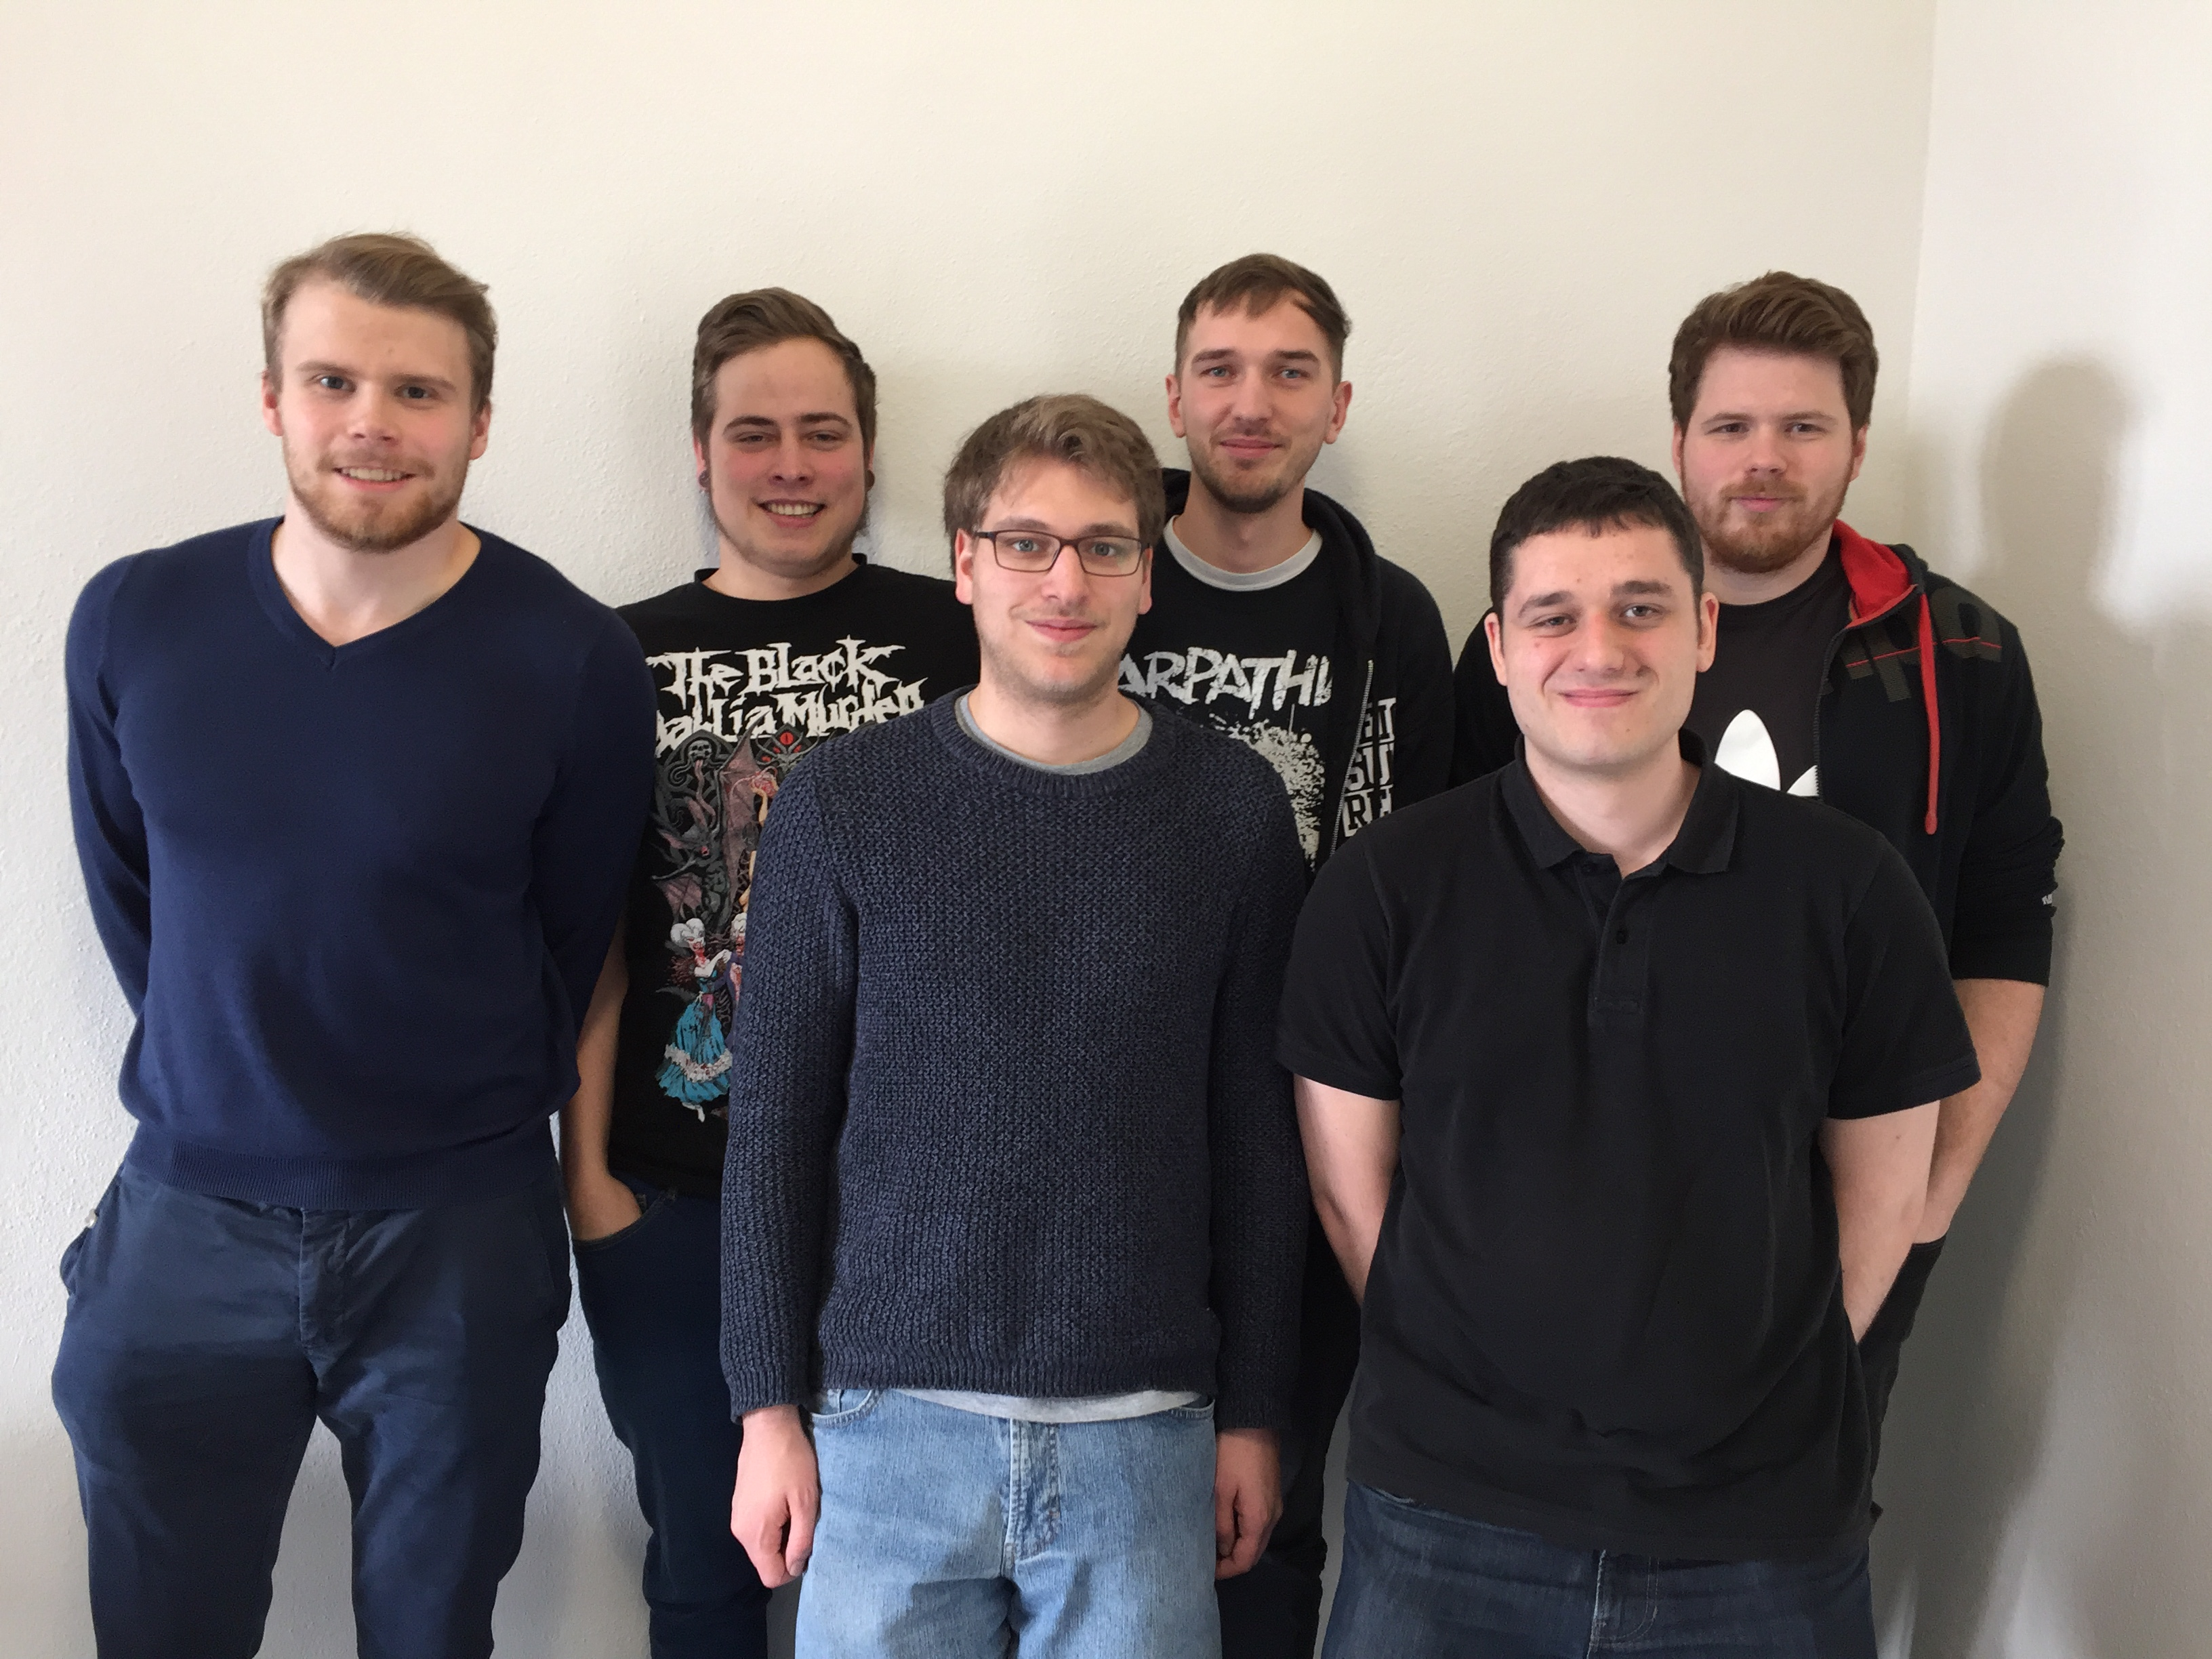
\includegraphics[height=12cm, width=15cm, keepaspectratio]{Gruppe.jpg}
\caption{Gruppe}
\end{figure}

\newpage
\section{Aufgabenstellung}

\begin{description}
   \item[Schwerpunkte des Projektseminars]~\par
   \begin{enumerate}
      \item Vorstellung und Diskussion von In-Memory-Technologien unter dem Aspekt der Hochverfügbarkeit und Performancesicherung.
      \item Erarbeitung von Strategien für die Umsetzung von Anforderungen an Konsistenz, Verfügbarkeit, Performance und Ausfalltoleranz (CAP)\\ bei verschiedenen Systemen für die Verwaltung transaktionaler Daten einerseits und die Analyse großer Datenmengen andererseits.
      \item Einarbeitung in die In-Memory-Funktionalitäten von SAP HANA Express und MS SQL Server 2016 hinsichtlich (alter und)\\ neuer Features zur Sicherung von Hochverfügbarkeit und/oder Performance.
      \item Untersuchung der Möglichkeiten von Cache-/In-Memory-Technologien\\ bei NoSQL-Datenbanken (z.B. Memcached).
      \item Erarbeitung eines konzeptionellen Entwurfs für ein mögliches Beispielszenario.
      \item Prototypische Umsetzung von In-Memory-Technologien an mehreren Beispielsystemen (vergleichende Analyse).
      \item Aufbereitung und Auswertung der Ergebnisse.
   \end{enumerate}
   
\end{description}
\newpage
\section{Theorie}
\subsection{Grundlagen In-Memory Technologie}
Der wichtigste Unterschied von einem In-Memory Datenbanksystem gegenüber einem herkömmlichen ist, dass die Datenhaltung im Hauptspeicher des Rechners erfolgt. Das führt zu erheblichen Vorteilen bei der Performance, da die Zugriffszeit so enorm verkürzt wird und Zugriffsalgorithmen sind einfacher. Nachteil ist vor allen der wesentlich höhere Preis für Arbeitsspeicher als für Festplatten. Da aber auch die Preise für jene mit ausreichender Speicherkapazität inzwischen nicht mehr unbezahlbar sind, werden In-Memory Datenbanken immer beliebter. Erst mit der Entwicklung der Kapazität der Hauptspeicher im letzten Jahrzehnt wurde es möglich In-Memory basierte Systeme zu schaffen. Wichtigste Voraussetzung dafür war die Entwicklung von 64 Bit Systemen. Durch diese wurde es möglich ausreichend großen Arbeitsspeicher zu entwickeln. Im allgemeinen gilt für Speicherarchitekturen, dass je langsamer sie sind, desto billiger werden sie. Zuletzt veränderte sich zwar auch der Rest der Speicher grundlegend durch den Einzug von SSD Festplatten (Flash-Speichern), die wesentlich schneller sind als die Hard Disk. Allerdings sind diese aus Sicht der Software immer noch eine Platte wegen der Persistenz und der Nutzungseigenschaften. Dies hat zur Folge, dass für den Zugriff auf diese immer noch die gleichen Methoden verwendet werden wie für die Hard Disks. Zur vollen Ausnutzung der Geschwindigkeit des Flash Speichermediums müssen diese Algorithmen ständig erneuert werden. Der Hauptspeicher hat dagegen den Vorteil, dass ein direkter Zugriff möglich ist. So dauert das sequenziellen Lesen von einem MB hier nur 250000 ns gegenüber 1851851,9 ns bei einer aktuell schnellen SSD und 30000000 ns bei einer Hard Disk. Alle normalen Operationen der Datenbank werden deshalb im Hauptspeicher ausgeführt und die Festplatte wird nur für Backups bzw. als Archiv genutzt. Als Problem ergibt sich, trotz der wesentlich besseren Performance ein Bottleneck beim Lader der Daten vom RAM in den Cache. \\Einhergehend mit der Datenhaltung im Hauptspeicher gibt es einer weitere wesentliche Änderung gegenüber konventionellen Datenbanksystemen. So erfolgt die Datenhaltung spaltenorientiert. Dabei werden alle Reihen (Tupel) in angrenzenden Blöcken gespeichert. Dadurch eignen sie sich perfekt für einen schnellen lesenden Zugriff, was beispielsweise für die Aggregation sinnvoll ist. Zur Reduzierung der Datenmenge werden bei In-Memory Datenbanksystemen verschiedenen Kompressionsverfahren genutzt. \\ Aufgrund der Datenhaltung im Hauptspeicher ergibt sich noch ein Nachteil aus ökologischer und ökonomischer Sicht. So ist der Energieverbrauch einer von Main-Memory Datenbankmanagementsystemen erheblich viel höher als der von konventionellen. So verbraucht ein "`System"' ganze 1,5 Megawatt. 

\subsection{Verwendete Datenbanksysteme}
\subsubsection{MS SQL Server}
Micorsoft SQL Server ist Datenbankmanagementsystem von Microsoft und auch eines der bekanntesten mit einem sehr weiten Verbreitungsgrad. Die erste Version wurde bereits in Kooperation mit der Firma Sybase 1989 veröffentlicht. Seit 1995 ist er in eigenständiger Entwicklung bei Microsoft. Eigentlich handelt sich es hier um ein klassisches relationales Datenbanksystem. Seit der Version 2014 stehen allerdings eine Reihe an IN-Memory Funktionen unter dem Namen "`In-Memory OLTP"' zur Verfügung. So ist es jetzt mögliche einzelne/ mehrere Tabellen speicheroptimiert ("`memory-optimized"') anzulegen. \\ Speicheroptimierte Tabellen werden als Objekte der Programmiersprache C gehalten. Diese sind so implementiert, dass eine Anwendung genauso auf sie zugreifen kann, wie auf eine althergebrachte Tabelle im Dateisystem.\\ Klare Vorteile dieser Tabellen sind die Möglichkeit wesentlich schneller arbeiten zu können, wie auch eine Multiversionsverwaltung. Dies bedeutet, dass wenn mehrere Transaktionen auf dieselben Datensätze zugreifen, eine eigenständige Version dieser verwendet. Dadurch fallen Sperren weg. Negativ ist, dass unter Umständen Datenverluste durch die Datenhaltung im Hauptspeicher entstehen können, da es verschiedene Beständigkeit dieser Tabellen gibt. So kann man Tabellen mit beständigen und mit nicht beständigen Inhalten erstellen. Bei letzteren erfolgt keine zusätzliche Sicherung auf der Festplatte, weshalb die Daten verloren sind, wenn es zu einem Ausfall, Neustart oder ähnlichen des Servers kommt.\\ Wird nun eine neue Tabelle mit beständigen Inhalt angelegt, erstellt MS SQL Server eine speicheroptimierte Dateigruppe mit einem Container. Dieser enthält Datendateien und Änderungsdateien. In der Dateigruppe erfolgt die zwischen Speicherung der Daten aus dem Arbeitsspeicher als Backup-Lösung. Eine speicheroptimierte Dateigruppe ist erforderlich, damit die Behandlung speicheroptimierter SCHEMA-ONLY-Tabellen für Datenbanken mit speicheroptimierten Tabellen konsistent ist. \\ Anfangs gab es noch zahlreiche Einschränkungen bei speicheroptimierten Tabellen. So waren SQL Befehle wie ALTER, LEFT/ RIGHT OUTER JOIN,1 OR, NOT, SELECT DESTINCT und einige andere nicht nutzbar, der maximal nutzbare Speicher auf 256 GB limitiert, Lagre Objects (LOBs) und einige weitere Dinge nicht unterstützt. Dies wurde mit der Version 2016 behoben. Der nutzbare Speicher wurde auf 2 TB erhöht. 
 
\subsubsection{SAP HANA}
Bei SAP Hana handelt es sich um eine komplette In-Memory Datenbanksystem aus dem Hause SAP. Es wurde erstmalig 2010 vorgestellt und setzt sich seit dem immer weiter durch. Entwickelt wurde es von dem Hasso-Plattner-Institut in Kooperation mit der Stanford University aus den USA. In einigen Veröffentlichungen, wie auch einem hier stark als Quelle genutzten Buches, wurde es auch als "`NewDB"' oder "`SanssouciDB"' bezeichnet. In unserem Projektseminar nutzten wir die Express Version die im Jahre 2016 veröffentlicht wurde. Sie ist bis zu einer Arbeitsspeicherkapazität von 32 GB. SAP plante sie um sie in Umgebungen einzusetzen wo nur eingeschränkte Ressourcen zur Verfügung stehen. Im Gegensatz zum Microsoft SQL Server wird bei SAP Hana die komplette Datenbank im Hauptspeicher gehalten und durch spezielle Sicherungsverfahren werden laufend Änderungen auf der Festplatte repliziert, sodass kein Datenverlust entsteht (Recoverystrategien). Es handelt sich hier um eine spaltenorientierte Datenbank. Betrieben werden kann SAP Hana Express entweder fest auf einem Server, auf einer VM oder seit neustem auch in der Cloud (z.B. Amazon Webservices oder Microsoft Azure). Unterstützt werden Server mit SUSE oder Red Hat Linux. Will man die 32 GB Begrenzung umgehen, so ist dies gegen eine Gebühr gestaffelt möglich. Sie lässt sich mit dem Hana Studio oder über eine Weboberfläche bedienen, wobei wir das Hana Studio genutzt haben, was auf der Eclipse Plattform basiert. Für das Datenbankmanagement stehen viele Möglichkeiten zur Verfügung. Neben der Spaltenorientierung "`Multi-Core"' und Parallelisierung, erweiterte Komprimierungsverfahren, "`Multi-Tenancy"', Möglichkeiten zur Datenmodellierung, Sicherheitskonzepte, sowie eine Offenheit. Daneben lässt sich noch  Anwendungsentwicklung, "`Advanced Analytical Processing"', sowie Datenintegration und Qualitätssicherung betreiben. Bei letzteren Daten Virtualisierung, ETL, Replikationen sowie eine Hadoop und Spark Integration. In der Express Version fehlen allerdings Funktionen wie "`Multi-Tier-Storage"', Hochverfügbarkeit und Katastrophenmanagement ebenso wie die Funktion zur Qualitätssicherung und zur Datensynchronisation (remote). Positiv ist ganz klar, dass sie sowohl für OLTP wie auch OLAP geeignet ist. Verfügt der Server mehr als 32 GB Arbeitsspeicher, lässt sich SAP Hana Express natürlich weiterhin anwenden, die Datenbankgröße ist lediglich auf 32 GB begrenzt.   
\subsubsection{Cassandra}
Cassandra ist ein sehr einfaches verteiltes Datenbanksystem. Im Gegensatz zu konventionellen Datenbanksystemen, wird hier auf No SQL gesetzt. Dies steht für "`Not only SQL"' und ist ein alternatives, nicht-relationales Datenbankmodell. Verwendet wird es überwiegend in Key-Value Datenbanken, Graphendatenbanken, dokumentenorientierte Datenbanken oder wie hier spaltenorientierten Datenbanken. NoSQL ist gekennzeichnet durch eine horizontale Skalierbarkeit, das Vermeiden unnötiger Komplexität, eine hohe Performance sowie ein hoher Datendurchsatz. Weiterhin werden relationale Ansätze des Datenmappings vermieden und es erfolgt eine einfache Replikation der Datenbanken. Schwächen liegen im einen Mangel einer umfangreichen Dokumentation. Es ist außerdem keine universelle Sprache wie SQL, es gibt immer wieder unerwartete Verhaltensweisen und fehlenden Support. \\ Heute ist Cassandra die populärste spaltenorientierte NOSQL-Datenbank. Große Firmen wie Apple, Netflix und Twitter nutzen sie und setzen dabei auf die Stärke, wie eine einfache horizontale Skalierbarkeit, eine hohe Ausfallsicherheit, die Unterstützung mehrere Datacenter und die Speicherung großer Datenmengen.\\ Sie besitze eine IN-Memory Funktion. Dabei ist eine parallele Nutzung von Standardtabellen und IN-Memory Tabellen, sowie ein blitzschneller Lesezugriff auf die Daten möglich. Cassandra eignet sich dadurch optimal bei read-only Zugriffen und konstanten Daten. 
\subsubsection{Maria DB in Kombination mit Memcached}
Maria DB ist ein kostenloses Datenbankmanagementsystem. Entstanden ist es aus einer Abspaltung von MySQL und wurde 2009 veröffentlicht. Im Gegensatz zu den anderen verwendeten Systemen handelt es sich hier um ein normales relationales Datenbanksystem. Es bietet also keine In-Momory Funktionalität und eben sowenig Spaltenorientierung. Sie dient hier dem Vergleich in Kombination mit Memcached.  
Memcached wurde entwickelt von Brad Fitzpatrick (Danga Interactive /  LiveJournal)und ist seit 15. Juni 2003 unter BSD-Lizenz verfügbar.
Viele große Unternehmen setzen auch hier wieder auf die Software wie zum Beispiel Facebook, Youtube oder Reddit. Hierbei handelt es sich um eine Server Applikation die Speicher im Arbeitsspeicher zur Verfügung stellt. Sie lässt sich über das Netzwerk oder das Internet ansprechen und kann Daten aufnehmen und auch zurückgeben. \\ Der größte Anwendungsbereich des Systems sind Webanwendungen. Es wird vor allem genutzt um einen schnellen Zugriff auf im Cache abgelegte Daten zu erhalten. Hier erfolgt eine Lastverteilung von Festplattenzugriffen und Datenbankanfragen auf den RAM. Es funktioniert dabei so, dass häufig abgefragte Daten (wie die Ergebnisse einer SELECT Abfrage) direkt im Arbeitsspeicher festgehalten werden, was wiederum erheblich kürzerer Antwortzeiten ermöglicht, da keine unnötigen Festplatten- und DBMS Zugriffe durchgeführt werden müssen. Ziel der Software ist die Optimierung der Antwortzeiten von Webanwendungen. \\ Memcached stellt dabei mehrere Hashtabellen zur Verfügung (Key-Tabelle und Hashtabelle). Es ist von der Funktionsweise vergleichbar mit assoziativen Arrays in verschiedenen Programmiersprachen. Memcached ist eine Hash-Tabelle und speichert die Daten in einer Key / Value Abhängigkeit ab. Dabei werden die Schlüssel und die Werte als Zeichenketten abgespeichert. Da von verschiedenen Programmen auf Memcached zugegriffen werden kann, ist es diesen möglich die Daten vor dem absenden an Memcache zu serialisieren. Somit können auch andere Datentypen wie Ganzzahlen, Fließkommazahlen und Objekte abgespeichert werden. Die Speicherverwaltung erfolgt über eine Slab-Allocator. Dies bedeutet, dass viele kleine Speicherbereiche häufig reserviert und wieder freigegeben werden. Diese sind dabei maximal ein Megabyte groß. Definierte Clients existieren hier nicht, wobei die Programm Bibliotheken sehr großen Einfluss nehmen. Am weitesten verbreitet ist die für PHP (PECL Memchached). \\Memcached-Server lassen sehr gut dezentralisieren. Dabei müssen diese  als Cluster zusammengeschlossen werden, um so den Arbeitsspeicher mehrerer Web-Server effizienter nutzen zu können. Wobei zu beachten ist, das die einzelnen Knoten keinen gemeinsamen Master-Knoten über sich haben. Dies muss von den Client-Bibliotheken übernommen werden, die entsprechend die Verteilung von Daten an die Memcached-Server überwachen muss. \\ Memcache Server antworten jedem Nutzer der Zugriff auf das System besitzt. Daher sollten Vorsichtsmaßnahmen ergriffen werden. Die Key’s sollten möglichst schon vom eigenen Programm verschlüsselt werden und erst danach an den Speicher abgegeben werden.



\newpage 
\subsection{In-Memory Technologie im Vergleich zur konventionellen Datenhaltung}
Die Speicherung in In-Memory Datenbanken erfolgt spaltenorientiert, was einer der größten Unterschiede im Vergleich zu konventionellen Datenbanken ist. Die Notwendigkeit zu diesem neuen Speicherverfahren resultiert aus dem extrem schnell wachsenden Berg an unstrukturierten Daten. Dies lässt sich vor allen im Internet beobachten wo es zu einem enormen Wachstum solcher Daten gekommen ist. 
In spaltenorientierten Datenbanken (mitunter auch als Wide Column Stores bezeichnet) erfolgt die Speicherung der Daten in Spalten und nicht in Zeilen. Die Einträge in einer Spalte bestehen dabei jeweils aus dem Namen, den Daten und dem Zeitstempel. Untergliedert wird dabei in "`Column Families"'. Das sind die Spalten mit gleichartigen, sich ähnelnden Inhalt die eine Tabelle bilden. 
Ein weiterer großer Unterschied ist, dass es innerhalb einer "`Column Family"' keinerlei logische Struktur existiert. Man bezeichnet sie deshalb auch als "`Wide Columns"'.  
Die Daten sind aus Sicht das Betriebssystem in einer eindimensionalen Folge von Bytes angeordnet. Bei einer zeilenorientierten Datenbank werden alle Datenwerte einer Zeile aneinander gehängt. Im Gegensatz dazu werden die Datenwerte einer spaltenorientierten Datenbank Spalte für Spalte aneinander gehängt.
Das führt zu einer Beschleunigung der Datenbereitstellung, da die Festplattenzugriffe verringert werden.
Das bringt Vorteile mit sich bei Anwendung wo z.B. Aggregate über große Zahlen oder ähnliches gebildet werden. Wenn ein Aggregat über viele Zeilen, aber nur wenig Spalten gebildet werden muss, kann man nun nur die gesuchten Spalten auslesen aber nicht mehr alle wie bei zeilenorientierten Datenbanken. Außerdem ist es effizienter wenn eine Spalte über alle Zeilen der Tabelle einen neuen Wert erhält, da man keine Rücksicht auf die Inhalte der anderen Spalten nehmen muss und so effizient schreiben kann.
Ein weiterer Vorteil ist das sich die Spalten orientierten Systeme sich selbst indexieren und so weniger Speicherplatz benötigt wird.
In der Praxis sind Spalten orientierte Systeme gut für OLAP- Aufgaben geeignet, da diese durch eine kleine Anzahl sehr komplexer Abfragen über alle Datensätze definiert sind.

\newpage
\subsection{Kompressionsverfahren}
Aus dem neuen Performance Bottleneck zwischen Hauptspeicher und Cache ergibt sich die Notwendigkeit Komprimierungsverfahren zu nutzen um eine  schnellere Arbeit zu gewährleisten. Weiterhin sind diese notwendig, da trotz der aktuell relativ großen Arbeitsspeicherkapazitäten die Datenbanken oft noch größere Mengen an Daten enthalten, weshalb ohne Komprimierung eine Datenhaltung im Hauptspeicher nicht möglich wäre. 
\subsubsection{Kompressionsverfahren bei SAP HANA}
Basis für die sehr effiziente Kompression stellt hier die spalten-orientierte Speicherung dar. Durch die Verringerung von Bits die zur Darstellung der Daten genutzt werden kann sowohl die Zugriffszeit, als auch der Speicherverbrauch verringert werden.\\
Grundlage stellt in der HANA das "`Dictionary Encoding"' dar. Dabei werden Werte mit einer großen Länge (wie Texte) als Integer Wert gespeichert. Dabei ist es einfach zu verstehen und nicht schwer zu implementieren, was zu höheren Vorteilen in der Performance führt. Es arbeitet dabei spaltenweise. Hat die Tabelle zum Beispiel eine Spalte fName, so wird hier jedem Vornamen eine Positionsnummer zugeordnet. In dem sogenannten "`Dictionary"' werden nun die Namen jeweils einzeln eingetragen und ebenso mit IDs versehen. Die beiden IDs werden dann einfach ein einem "`Attribut Vector"' verknüpft. Je mehr Dopplungen von Namen in der Spalte fname sind, desto höher ist die Komprimierung. Angenommen jeder Vorname besteht aus 49 Byte und es gibt acht Milliarden Menschen auf der Erde, dann werden rund 365,1GB benötigt um alle zu speichern. Dahingegen braucht der "`Attribut Vector"' 23 Bit pro Eintrag multipliziert mit den 8 Millionen Einträgen also 184 Milliarden Bit, was 21,4GByte entspricht. Das "`Dictionary"' verbraucht bei 49 Byte pro Eintrag  und 5 Millionen Vornamen nur 0,23GByte. Dividiert man nun die Menge ohne Kompression von 365,1GByte mit den 21,63GByte nach Kompression, sieht man, dass man der Speicherverbrauch um den Faktor 17 gesunken ist, was 6 Prozent des ursprünglichen Speicherbedarfs darstellt. Nutzt man dieses Prinzip bei den Geschlechtern,über ebenfalls 8 Milliarden Menschen, werden nur noch 0,93GB anstelle von 7,45 GB benötigt (Kompressionsfaktor 8). Der Kompressionsfaktor hängt dabei von der Größe der Daten sowie der Tabelle ab, also der Spaltenkardinalität und der Tabellenkardinalität (Entropie - Maß für Informationsgehalt). Ein weiterer Geschwindigkeitsvorteil lässt sich durch sortierte "`Dictionarys"' errreichen, da dann Binärsuche angewendet werden kann. Nachteil dieser Sortierung ist, das sie immer wieder neu durchgeführt werden muss, sobald ein Wert in dem "`Dictionary"' angefügt wird. Dies verursacht bei großen, sich ständig ändernden Datenmengen, aber wieder erhebliche Kosten. \\ Ein sehr großer Vorteil dieser Methode ist außerdem, dass alle Operationen auf den Daten der Tabelle in Attributvektoren mit Integer Werten ausgeführt werden. Diese kann der Prozessor wesentlich schneller verarbeiten als Zeichenketten. Der Prozessor muss so zwar eine Zusatzlast stemmen, aber da der Arbeitsspeicher hier der Bottleneck ist, ist dies vertretbar und fällt nicht sehr ins Gewicht. Da in der Regel die Ergebnismenge kleiner als die komplette Tabelle ist und bei vielen Operationen wie z.B. "`Count"' nicht die echten Werte benötigt werden, ergibt sich auch kein Nachteil aus dieser Methode. \\ Da die Datenbanken großer Unternehmen oft mehrere Terabyte groß sind und die Kapazität der Arbeitsspeicher noch weit darunter ist, werden zusätzlich noch Kompressionsverfahren genutzt um ganze Datenbank im Hauptspeicher halten zu können. Dies hat auch den Vorteil, dass weniger Daten zwischen dem Prozessor und dem Speicher fließen müssen, was wiederum die Performance verbessert. Wichtig ist hier das Verhältnis von Kompression und den zusätzlich benötigten Operationen des Prozessors. \\ Heutige Datenbanken enthalten oft "`tonangebende"' Werte, wodurch derselbe Wert ohne Komprimierung sehr oft gespeichert werden muss. Um dieses Problem zu beheben und Speicher einsparen zu können wird das sogenannte "`Prefix Encoding"' genutzt. Dafür müssen die Daten nach besagtem Wert sortiert werden und der Attributvektor mit diesem starten. Bei dem Verfahren wird nun nur eine Instanz des Wertes und die Häufigkeit dessen im "`Attribut Vector"' gespeichert, anstelle des Wertes in doppelter und dreifacher Ausführung. Der Vektor besteht dann aus der Häufigkeit des Wertes, der ID aus dem "`Dictionary"' und der ID's der folgenden Werte. Nimmt man nun zum Beispiel die Tabelle mit der Bevölkerungsmenge nach Ländern sortiert, so befand sich der Wert für China ungefähr 1,4 Milliarden mal in dem "`Attribut Vector"'. Daraus ergibt sich ein Speicherbedarf von 1,4 Milliarden mal 8 Bit. Mit "`prefix Encoding"' lässt sich dies auf nur 39 Bit verringern (8 Bit für das einmalige Speichern und 31 Bit für die Häufigkeit). Darauf ergibt sich eine Ersparnis von immerhin 17 Prozent (1,3 GByte in diesem Beispiel). Zusätzlich dazu ermöglicht es direkten Zugriff über "`row number claculation"' (Dabei determiniert die Datenbank, dass nur die bestimmte Anzahl an Zeilennummern benötigt (im Beispiel 1 - 1,4 Milliarden), was zu schnelleren Ergebnissen führt. \\ Eine weitere Möglichkeit der Kompression bietet das "`Run Length Encoding"'. Es funktioniert am besten, wenn der "`Attribut Vector"' einige sich unterscheidende Werte enthält, die sich sehr oft wiederholen. Zur Erreichung besonders guter Ergebnisse, muss die Spalte (des Vektors) sortiert werden. Die beieinanderliegenden gleichen Werte werden nun wieder zu einem zusammengefasst mit entweder der Häufigkeit oder der Startposition als Abstände. Letzteres hat dabei den Vorteil, dass ein schnellerer Zugriff ermöglicht wird, da direkt die Adresse eines Wertes gelesen werden kann, anstatt das diese erst berechnet werden muss. Bezogen auf das obige Beispiel lässt sich bei der Länderspalte wieder sehr viel einsparen. Dafür werden zwei Vektoren benötigt. Einer mit allen Ländern (200 Einträge) und einer mit den Startpositionen der einzelnen Länder. Acht Bit benötigt jeder Eintrag der Länder und 33 Bit jede Startposition (Log\textsubscript{2} 8.000.000.000) plus ein Extra Feld (33 Bit) am Ende, welches die Häufigkeit des letzten Wertes beinhaltet (da diesem ja kein neuer Wert folgt). Alles in allem ergibt sich eine Größe des Vektors von nur rund 1 KB gegenüber 7,45 GB [200*(33Bit + 8 Bit)+ 33Bit]. Würde man die Häufigkeit anstelle der Startposition nehmen, könnte man zwar nochmal 33 Bit einsparen, aber es wäre kein direkter Zugriff mehr möglich, was zu einer viel höheren Antwortzeit führen würde und daher keine gute Option für IN Memory Datenbanken ist.\\ Cluster Encoding ist ein weiteres Interessantes Kompressionsverfahren. Hier wird der "`Attribut Vector"' in Blöcke der gleichen Größe unterteilt (oft 1024 Werte). Befinden sich in einem Block nur gleiche Einträge, so werden diese zu einem zusammengefasst. Ist dies nicht gegeben, bleibt der Block unverändert. Nun wird noch ein zweiter Vektor benötigt in dem steht, welcher Block durch einen einzelnen Wert ersetzt wurde (wenn Block unverändert 0, wenn zusammengefasst dann 1). Um hier auf die  einzelnen Werte zuzugreifen, wird der Index mit Hilfe von Integer Division berechnet (Zeilennummer durch Größe des Blockes). Der wohl größte Nachteil ist hier, dass kein direkter Zugriff auf die Werte möglich ist. Es lässt sich aber eine große Menge Speicher einsparen. In Bezug auf das obige Beispiel, benötigt man bei der Spalte mit den Städten nur noch rund 2,4 GB, anstatt 18,6 GB (87 Prozent Kompressionsrate unter der Annahme, dass es 1 Million Städte gibt).\\ Bei "`Indirect Encoding"' wird der Vektor ebenso in eine Vielzahl gleich großer Blöcke unterteilt (Größe meist wieder 1024). Als sehr effektiv erweist sich diese Methode, wenn ein Block einige sich unterscheidende Werte enthält, was oft gegeben ist, wenn eine Abhängigkeit zwischen zwei Spalten existiert und die Tabelle nach einer sortiert wurde (z.B. nach Land sortiert, wenn man die Spalte Vorname betrachtet wird). Hier wird neben dem globalen "`Dictionary"' noch ein lokales benötigt. Wenn man nun die Spalte Vorname betrachtet und annimmt, dass es im Schnitt 200 verschiedene Vornamen in einem Block pro Land gibt, wird in dem lokalen Wörterbuch jedem Wert für einem Namen ein Wert von 0 bis 199 zugeordnet, dieser dann in einem Vektor gespeichert. Die Einsparung an Speicherplatz resultiert hier daraus, dass bei nur 200 verschiedenen Werten nur noch acht statt 23 Bit pro Eintrag belegt werden (Log\textsubscript{2}(5 Millionen verschiedenen Namen Global) ergibt 23 Bit pro Eintrag ohne Kompression), unter der Voraussetzung das vorher nach den Ländern sortiert wurde. Hier erreicht man z.B. immerhin eine Kompressionsrate von 44 Prozent (nur rund 11,8 GB und nicht 21,4 GB) und ein direkter Zugriff ist im Gegensatz zum "`Cluster Encoding"' weiterhin möglich.\\ Neben der Verringerung der Größe des "`Attribut Vectors"' gibt es noch die Möglichkeit das "`Dictionary"' zu optimieren. Das wird mit "`Delta Encoding"' erreicht. Ist es nun alphanumerisch sortiert gibt es oft viele Werte mit der derselben Vorsilbe. Diese Tatsache macht man sich hier zu Nutze indem gemeinsame Vorsilben nur ein Mal gespeichert werden. Dabei wird wieder Blockweise gearbeitet ( oft mit 16 Strings pro Block). es speichert die Länge der ersten Zeichenkette, gefolgt von dieser am Anfang eines Blocks. Bei den darauffolgenden Werten wird nun die Anzahl an Zeichen die gleich dem Vorgänger sind gespeichert plus der Anzahl an folgenden, gefolgt von eben diesen Zeichen. Nimmt man zum Beispiel die Städte im "`Dictionary"', der erste Wert des Blocks ist Aach gefolgt von Aachen, dann wird im komprimierten Vektor die Länge 4 und die Zeichen von "`Aach"' festgehalten. Für "`Aachen"' wird die Länge der gleichen Teils "`Aach"' mit der 4 ersetzt, dann die Anzahl der folgenden und die Zeichen an sich gespeichert "`en"'. Dies lässt sich dann immer weiter so aufbauen, was im optimalen Fall immer mehr Einsparung mit sich bringt. Im hier betrachteten Beispiel mit den Städten wird eine Kompressionsrate von 90 Prozent erreicht ( rund 5,4 MB gegenüber 46,7 MB). \\ Bei al den Vorteilen durch Kompression sind dem Ganzen auch Grenzen gesetzt. So werden für die meisten Verfahren sortierte Tabellen benötigt um maximale Erfolge zu erzielen, aber es kann in einer Tabelle immer nur nach einer Spalte sortiert werden. Wenn kein direkter Zugriff möglich ist, ergibt sich außerdem ein großer Nachteil in der Performance.
\newpage
\subsubsection{Kompressionsverfahren bei MS SQL Server}
Auch der MS SQL Server verwendet für die Datenhaltung in speicheroptimierten Tabellen Kompressionsverfahren. Leider wird dazu nichts öffentlich kommuniziert. Es ist nicht bekannt, welche dort verwendet werden. 
\subsubsection{Kompressionsverfahren bei Cassandra}
Cassandra verwendet zur Datenspeicherung SSTables(Sorted String Tables) welche unveränderlich im Speicher abgelegt werden. Werden Daten verändert, so wird nicht wie bei traditionellen relationalen Datenbanken eine Dekomprimierung mit anschließendem Überschreiben und Komprimieren der Daten durchgeführt, sondern weitere SSTable im Speicher abgelegt, welche dann von Zeit zu Zeit mit bereits bestehenden SSTables verglichen und verbunden werden um Daten aktuell zu halten und Speichernutzung zu minimieren.
Datenbanktabellen können mittels verschiedener Verfahren komprimiert werden. 
\begin{description}
	\item[Cassandra unterstützt dabei folgende Komprimierungsverfahren:]~\par
	\begin{itemize}
		\item LZ4-Komprimierung
		\item Snappy-Komprimierung
		\item Deflate-Komprimierung
	\end{itemize}
\end{description}
Man kann sowohl beim Erstellen von Tabellen als auch beim Verändern festlegen, welche Methode zum Komprimieren verwendet werden soll.
\begin{verbatim}
CREATE TABLE Tabelle1(
                                            …
                                           )
WITH compression = { ‘class’ : ‘LZ4Compressor’|‘DeflateCompressor’|‘SnappyCompressor’ };
ALTER TABLE Tabelle1
WITH compression = { ‘class’ : ‘LZ4Compressor’|‘DeflateCompressor’|‘SnappyCompressor’ };
\end{verbatim}
Somit ist es möglich das Komprimierungsverfahren an die in der Tabelle geführten Daten anzupassen oder sogar zu deaktivieren. 
Der Algorithmus den die Snappy-Komprimierung verwendet ist auf hohe Komprimierungs- und Dekomprimierungsgeschwindigkeit ausgelegt mit einer folglich schlechteren Komprimierungsrate. 
Die Deflate-Komprimierung zielt darauf hinaus Daten verlustlos zu komprimieren wie dies zum Beispiel bei ZIP-Dateien der Fall ist.
Die Stärken beider vorher genannten Verfahren werden in der LZ4-Komprimierung vereint. Hierbei werden extrem hohe Komprimierungs- und Dekomprimierungsgeschwindigkeiten (50-80 Prozent schneller im Vergleich zu an anderen Verfahren) mit einer verlustfreien Kompression verbunden und trotzdem eine sehr gut Kompressionsrate erreicht, weshalb LZ4 auch das am meisten verwendete Verfahren ist.



\subsubsection{Kompressionsverfahren bei Maria DB mit Memcached}
Da Memcached eine reine Speicherfunktion erfüllt, gibt es im Programm selber keine Methoden zur Komprimierung. Jedoch bieten viele der Bibliotheken eigene Kompressionsverfahren an, die auf die Daten angewendet und danach an den Memcached-Server übermittelt werden. Die PHP-Extension stellt zum Beispiel eine auf dem Deflate-Algorithmus basierende Kompressionsmethode zur Verfügung.


\subsection{Parallele Verarbeitung}
Die In-Memory Datenbanksysteme sind sowohl in der Lage in Einem PC-System als auch in mehreren PC-Systemen die Arbeitsschritte der Abfrage aufzuteilen und damit z.B. auf einzelnen Bereichen des Arbeitsspeichers bestimmte Teilsuchen oder Teilberechnungen durchzuführen und parallel auf anderen Bereichen andere Teilsuchen bzw. Berechnungen.
Dadurch können die Abfragen viel schneller bearbeitet werden.
Ein Beispiel zur Aufteilung der Arbeitsschritte auf Serverblades (Sehr kompakte Server):

\begin{figure}[H]
\centering
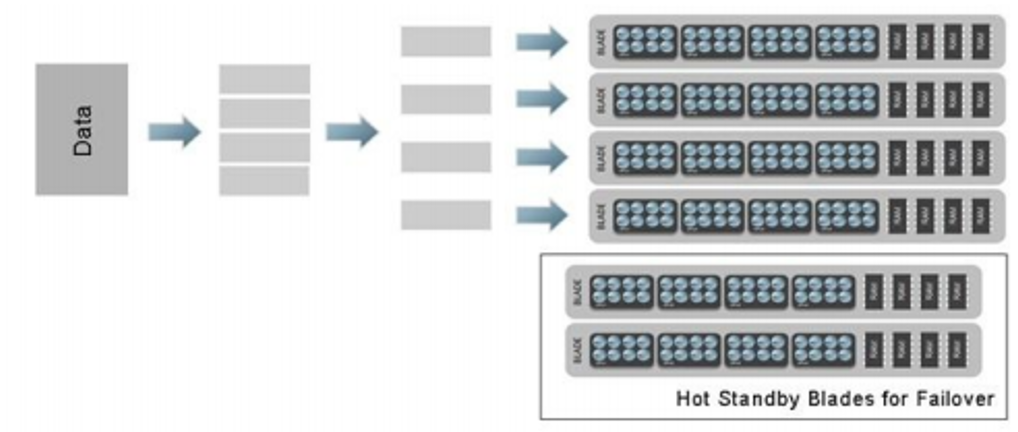
\includegraphics[height=12cm, width=17cm, keepaspectratio]{PrallelVer.png}
\caption{Parallele Verarbeitung}
\end{figure}  
Diese Aufteilung der Abfrage kann auch auf mehreren PC-Systemen/Servern stattfinden umso die Performance des Programms noch zu verbessern.
\subsubsection{Parallele Verarbeitung im MS SQL Server}
Bei MSSQL ermöglichen die parallelen Abfragen die Abfrageausführung und Indexvorgänge für Computer zu optimieren, die über mehrere Mikroprozessoren verfügen. 
MSSQL nutzt weiterhin mehrere Betriebssystemthreads für die Ausführung von Abfragen oder Indexvorgängen, so können diese effizient und schnell ausgeführt werden.
Um eine Abfrage optimieren zu können, sucht MSSQL erst mal nach Abfragen und Indexvorgängen die für eine parallele Ausführung vorteilhaft sind. Danach fügt es für diese Verteilungsoperatoren in denn Abfrageausführungsplan ein, damit bereitet es die ausgewählten Abfragen für die parallele Ausführung vor. Ein Verteilungsoperator ermöglicht die Prozessverwaltung, die Neuverteilung der Daten und die Ablaufsteuerung. Er schließt außerdem die Untertypen Distribute Streams, Repartition Streams und Gather Streams ein. 
Nachdem der Verteilungsoperator eingefügt wurde, ist das Ergebnis ein Plan für eine parallele Abfrageausführung. Dieser kann mehrere Threads verwenden, die genaue Anzahl der Threads wird während der Initialisierung definiert und durch die Komplexität des Plans und den Grad der Parallelität bestimmt. Der Grad der  Parallelität die maximal zu verwendete Anzahl an CPUs.

\subsection{Hochverfügbarkeit}
Die In-Memory Datenbank wird beim Erstellen und nach Transaktionen in Logdateien die in einer Containern Group sind auf der normalen Festplatte gespeichert.
Bei MSSQL beispielsweise musste diese Container Group vorm erstellen der Tabellen definiert werden.
\begin{verbatim}
ALTER DATABASE Testdatenbank ADD FILEGROUP Testdatenbank_mod CONTAINS 
MEMORY_OPTIMIZED_DATA   
ALTER DATABASE Testdatenbank 
ADD FILE (name=' Testdatenbank_mod1', filename='c:\data\Testdatenbank_mod1') 
TO FILEGROUP Testdatenbank_mod;

ALTER DATABASE Testdatenbank 
SET MEMORY_OPTIMIZED_ELEVATE_TO_SNAPSHOT=ON;  
\end{verbatim}
Dadurch kann die Verfügbarkeit der Daten auch Bei Systemausfall gewährleistet werden.
Die Logdateien dienen als Abbild der Datenbank und können diese jederzeit replizieren.
Die Hochverfügbarkeit kann bei In-Memory Datenbanksystemen wie bei normalen Datenbanken auch durch Storage Replication oder Logdateien auf separaten Servern etc. gesichert werden.



\newpage
\section{Anwendungsbeispiel}
Um einen möglichst realistischen Vergleich der Systeme durchführen zu können, haben wir uns ein Demoszenario ausgedacht, was uns als Datengrundlage dient. 
\subsection{Demoszenario}
Die Datenbank der RuckZuck Versandhaus GmbH. Diese hat eine Tabelle mit den Kunden, welche neben den allgemeinen Kundendaten wie Name, Vorname und Kundennummer noch zusätzliche Attribute wie das Beziehungslevel und der Person die den Kunden angeworben hat. Die Kunden geben beim Einkauf im Onlineshop eine Bestellung ab. Diese werden in der Tabelle Bestellungen genau gespeichert. In der befinden sich Informationen zur Bestellung wie die Bestellnummer, das Datum, die Artikelbezeichnung, Rabatte und auch die Kundennummer. \\ Das besondere an der RuckZuck Versandhaus GmbH ist, dass sie einen internen Versanddienst hat, der die Bestellungen direkt ausliefert. Dieser ist in verschiedenen Standorten in Deutschland aktiv. Diese sind auch erfasst. In der Tabelle Lieferdienst wird die Bestellnummer erfasst, ebenso wie die Liefernummer, der Preis und der Lieferstart.

\begin{figure}[H]
\centering
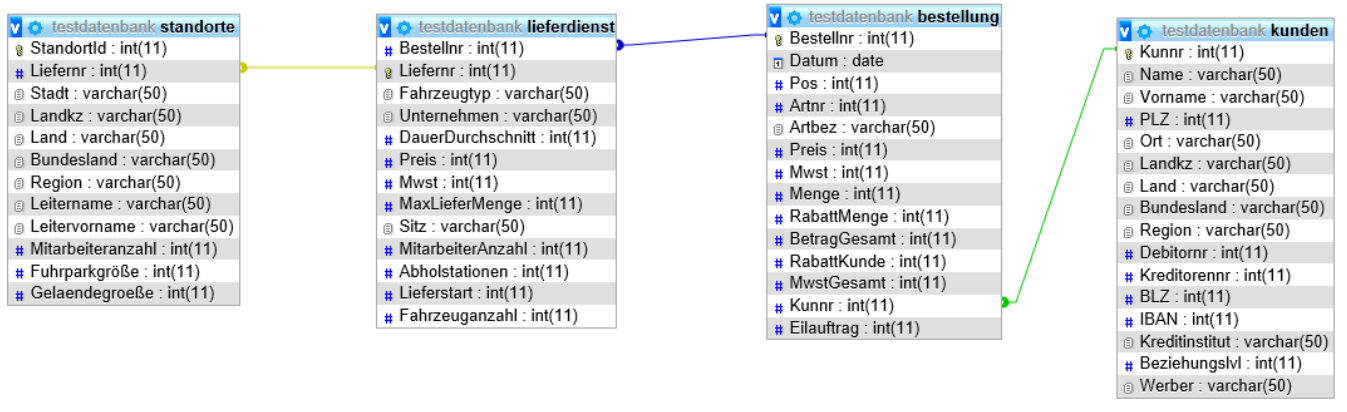
\includegraphics[height=4cm,width=0.8\textwidth]{DBUebersicht.PNG}
\caption{Tabellenstruktur}
\end{figure}
 
\subsection{Datengenerierung}
Wir haben nach einer Methode gesucht die Datenbank mit vielen aber auch sinnvollen Daten zu befühlen. Dabei sind wir auf  den "dbForge Data Generator" gestoßen.
In der dbForge haben wir als erstes die zu befüllenden Tabellen der Datenbank ausgewählt. Dann Haben wir für jede Spalte einen geeigneten Zufalls Wert ausgewählt. 
Zum Beispiel haben wir bei der Spalte Ort ausgewählt das er diese mit zufälligen Deutschen Städte Namen befühlt.
Nach dem wir dieses bei allen spalten getan haben, musste man nur noch auswählen wie viele Zeilen eingefügt werden sollen. Wir haben uns für 10 Millionen Zeilen entschieden und das Programm bis zum nächsten Tag arbeiten lassen. Daraus ergab sich eine gute Datengrundlage mit der wir weiterarbeiten konnten.


\subsection{Datenexport}
Damit wir in den anderen drei Datenbanksystemen die selbe Datengrundlage haben, mussten die befüllten Tabellen der MS SQL Server Datenbank als Flat Files exportiert werden. Dazu wurde der "`SQL Server - Import/Export - Assistent"' verwendet. Dort wird die gewünschte Tabelle ausgewählt, das Trennzeichen festgelegt und im nächsten Schritt noch als welche Datei exportiert werden soll. Wir setzen hier auf das CSV Format, da es von allen anderen Systemen unterstützt wird. 

\begin{figure}[H]
\centering
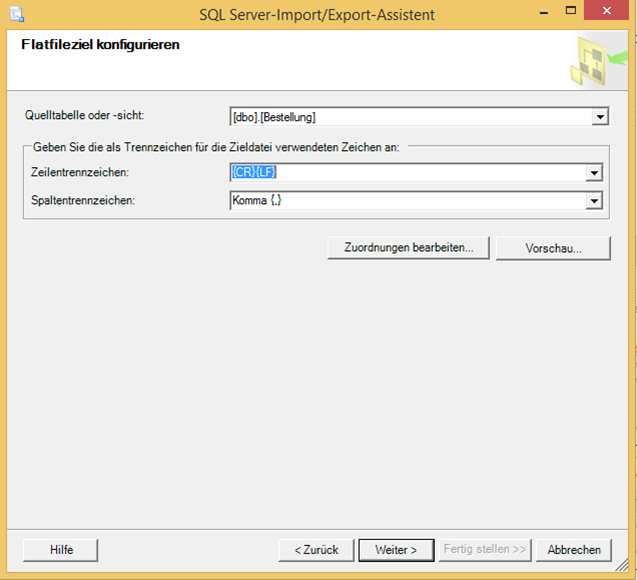
\includegraphics[height=12cm, width=15cm, keepaspectratio]{FlatExport.png}
\caption{Einstellungen Export als Flatfile}
\end{figure}

\begin{figure}[H]
\centering
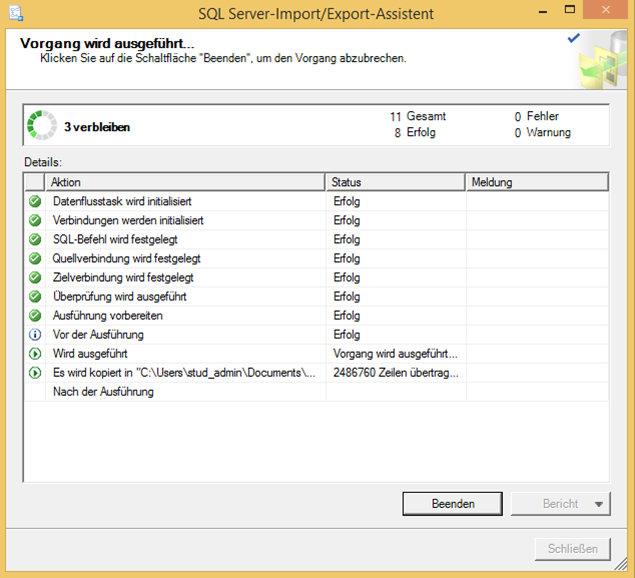
\includegraphics[height=12cm, width=15cm, keepaspectratio]{FlatExport2.png}
\caption{Prozess}
\end{figure}



\newpage
\section{Installation der Systeme}
\subsection{Aufsetzen des MS SQL Server}
\subsubsection{Installation des Servers}
Wir haben zunächst die Software heruntergeladen mit Hilfe unseres Zuganges als Studenten der Wirtschaftsinformatik zu Microsoft Imagine. 
Der MS SQL Server wurde standardmäßig installiert. Es mussten keine extra Einstellungen vorgenommen werden. 
\begin{description}
	\item[Vorgang]~\par 
	\begin{enumerate}
		\item Im Fenster des Installation Center unter dem Reiter "`Installation"' haben wir die Installation eines neuen SQL Servers gestartet. 
		\item Jetzt wurde der Instanz ein eigener Name vergeben. 
		\item Im nächsten Schritt wurde eingestellt, dass die Dienste automatisch gestartet werden, sodass wir diese nicht jedes Mal manuell einschalten müssen. 
		\item Da wir das System direkt auf dem Rechner im Labor verwendet haben, haben wir nur den "`Windows authentication mode"' genommen.
		\item Nachdem die Installation abgeschlossen war, haben wir die des SQL Server Managementstudios gestartet. Dieses wurde ebenso standardmäßig installiert. 
		\item Daraufhin wurde das Management Studio gestartet. Im Login Fenster haben wir bei "`browse for more"' unter dem Reiter "`Database Engine"' die zuvor angelegte SQL Server Instanz ausgewählt und uns dann mit der Windows Authentifikation angemeldet. 
		\item Nun wurde noch die Datenbank "`Testdatenbank"' angelegt. 
	\end{enumerate}
\end{description}

\subsubsection{Einrichten der Datenbank}
\begin{description}
	\item[Vorgehen]~\par 
	\begin{enumerate}
		\item Mit folgenden Statement haben wir die In-Memory Funktionalität der Datenbank aktiviert. 
		\begin{verbatim}
ALTER DATABASE Testdatenbank ADD FILEGROUP Testdatenbank_mod CONTAINS 
MEMORY_OPTIMIZED_DATA   
ALTER DATABASE Testdatenbank 
ADD FILE (name=' Testdatenbank_mod1', filename='c:\data\Testdatenbank_mod1') 
TO FILEGROUP Testdatenbank_mod;   
		\end{verbatim}
		Damit wurde eine speicheroptimierte Dateigruppe mit einem Container erstellt. Dieser enthält entweder Datendateien, Änderungsdateien oder beide. Eine speicheroptimierte Dateigruppe ist erforderlich, damit die Behandlung speicheroptimierter SCHEMA_ONLY-Tabellen für Datenbanken mit speicheroptimierten Tabellen konsistent ist.\\ 
		In dieser Dateigruppe erfolgt die Zwischenspeicherung der Daten aus dem Arbeitsspeicher (Backup-Lösung). 
		\item Nun musste Tabellenhinweis auf die speicheroptimierte Tabelle erstellt werden. Dabei muss der Hinweis für SNAPSHOT oder eine stärker isolierende Stufe erfolgen
		\begin{verbatim}
ALTER DATABASE Testdatenbank 
SET MEMORY_OPTIMIZED_ELEVATE_TO_SNAPSHOT=ON;  
		\end{verbatim}
		\item Die Tabellen wurden mit dem Verweis "`MEMORY_OPTIMIZED=ON"' erstellt, um sie als speicheroptimierte Tabellen anzulegen. 
		\begin{verbatim}
CREATE TABLE Bestellung 
(
Bestellnr int Primary Key NONCLUSTERED,
Datum date,
Pos int,
Artnr int,
Artbez varchar,
Preis int,
Mwst int,
Menge int,
RabatMenge int,
BetragGesamt int,
RabatKunde int,
MwstGesamt int,
Kunnr int,
Eilauftrag int
) WITH (MEMORY_OPTIMIZED=ON)

		\end{verbatim}
		Der "`Primary Key NONCLUSTERED"' stellt dabei einen nicht gruppierten speicheroptimierten Index bereit. \\ Analog wurde bei den anderen Tabellen vorgegangen.	
		
	\end{enumerate}
\end{description}
 






 
\subsection{Aufsetzen der SAP Hana Express}
Da SAP Hana Express nur auf Linux Systemen installierbar ist und unser Testsystem ein Windows Betriebssystem hatte, mussten wir uns mit einer VM behelfen.\\
Wir haben uns für die VMware Workstation 12 Pro Version: 12.5.0 build-4352439 entschieden. Für das DB-System haben wir schon eine ISO-Datei heruntergeladen.
\subsubsection{Installation}
\begin{description}
   \item[Einrichten der VM]~\par
   \begin{enumerate}
      \item Als erstes gehen wir mit Rechtsklick auf die ISO-Datei und öffnen diese mit der VM Workstation.Dadurch können wir die ISO-Datei importieren.
      
\begin{figure}[H]
\centering
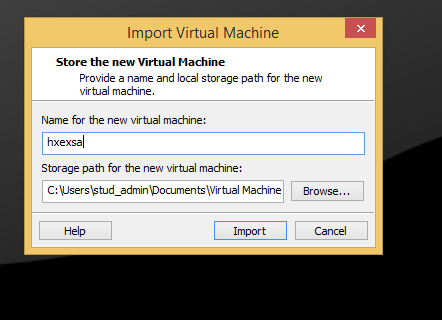
\includegraphics[height=12cm, width=15cm, keepaspectratio]{Hana1.png}
\caption{Neue VM}
\end{figure}
     \newpage
      \item Nun müssen ausreichend Ressourcen für die VM zugeteilt werden. Dabei ist besonders der Arbeitsspeicher relevant, da dort die Datenbank liegen soll.
      
\begin{figure}[H]
\centering
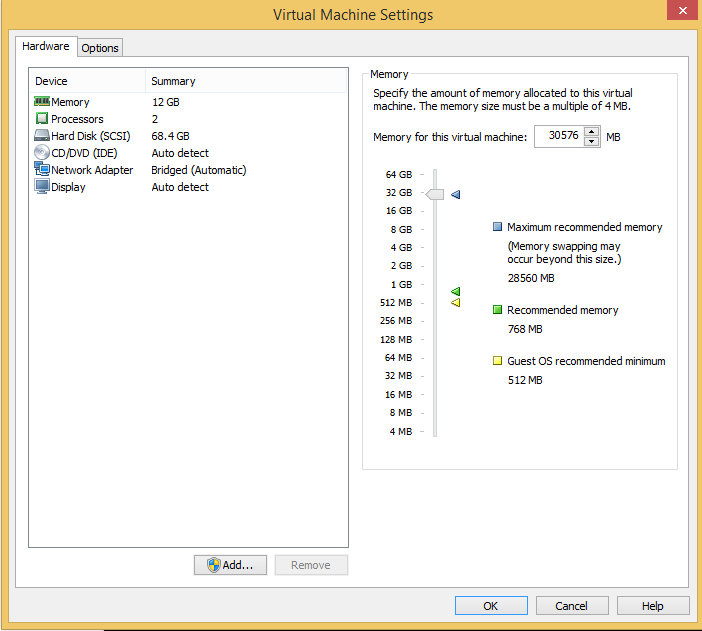
\includegraphics[height=12cm, width=15cm, keepaspectratio]{Hana2.png}
\caption{VM Settings}
\end{figure}

      \item Als "hxehost login" nehmen wir hxeadm und als Passwort HXEHana1 (Passwort nur temporär). 

\begin{figure}[H]
\centering
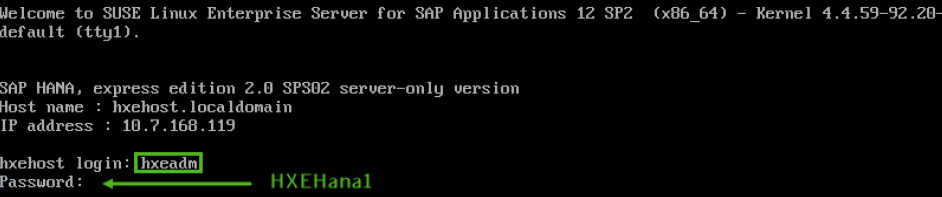
\includegraphics[height=12cm, width=15cm, keepaspectratio]{Hana3.png}
\caption{VM User}
\end{figure}
       
      \item Direkt danach können wir selber unser Passwort bestimmen.
      
\begin{figure}[H]
\centering
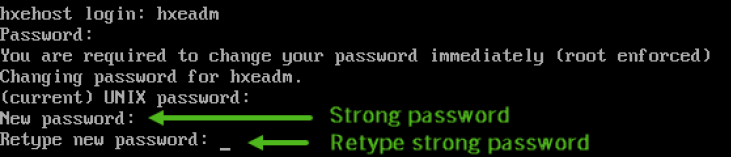
\includegraphics[height=12cm, width=15cm, keepaspectratio]{Hana4.png}
\caption{VM Passwort}
\end{figure}

      Das database master Passwort ist das selbst bestimmt Passwort.
      \item Danach muss in der Windows hosts Datei noch ein Vermerk zum Aufruf der Weboberfläche eingetragen werden. \\Windows->System32->drivers->etc

\begin{figure}[H]
\centering
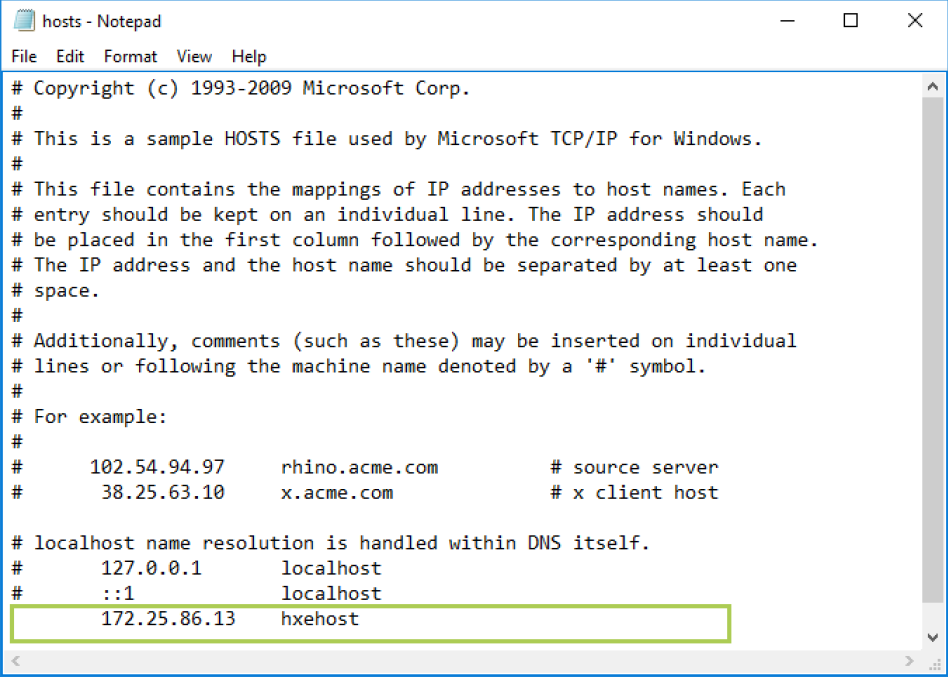
\includegraphics[height=12cm, width=15cm, keepaspectratio]{Hana5.png}
\caption{VM hosts}
\end{figure}      
\newpage
      \item In der VM den Befehl xs apps eingeben um zu schauen, welche Applikationen laufen. Wichtig ist hierbei die markierte Stelle. Die URL rechts notieren, damit man im Browser die GUI aufrufen kann.
      
\begin{figure}[H]
\centering
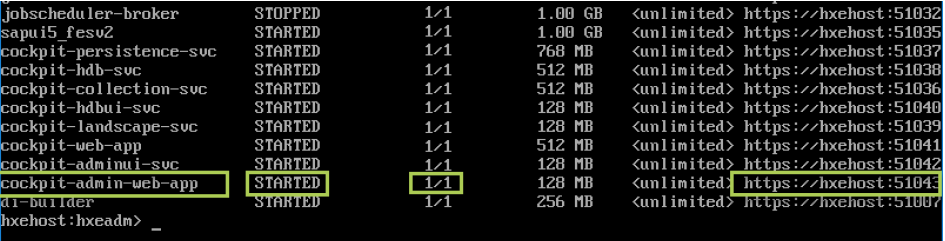
\includegraphics[height=12cm, width=15cm, keepaspectratio]{Hana6.png}
\caption{URL Webapp}
\end{figure}      
      
      
      Da wir die Web-GUI nicht genutzt haben sondern mit der Eclipse-Oberfläche gearbeitet haben, stellen wir jetzt die Arbeitsweise mit Eclipse vor. Um die Web-GUI zu bedienen empfiehlt sich folgendes Dokument von SAP HANA: https://www.sap.com/developer/tutorials/hxe-ua-getting-started-vm.html
      \item Nun Eclipse installieren (Eclipse Neon .3) und danach starten. Um im Eclipse mit SAP HANA express arbeiten zu können, muss noch ein weiteres Tool heruntergeladen werden. Dazu auf Help -> Install New Software… gehen. 

\begin{figure}[H]
\centering
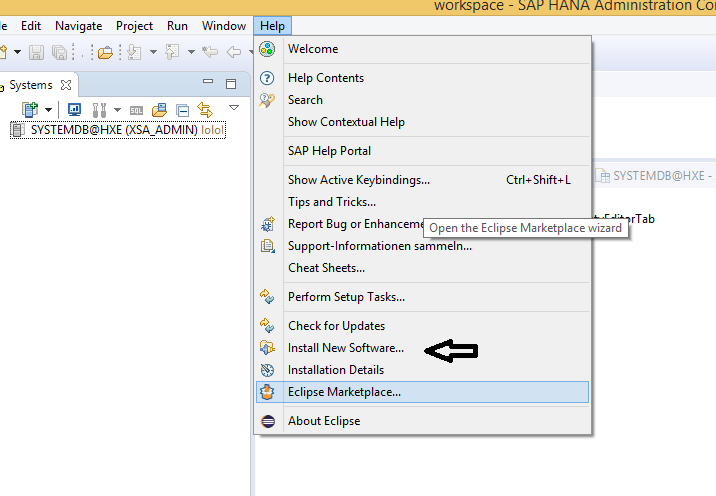
\includegraphics[height=12cm, width=15cm, keepaspectratio]{Hana7.png}
\caption{Eclipse new Software}
\end{figure}    

      \item Auf "`Available Software Sites"' klicken und im öffnendem Fenster auf den Reiter HANA gehen und Apply drücken.

\begin{figure}[H]
\centering
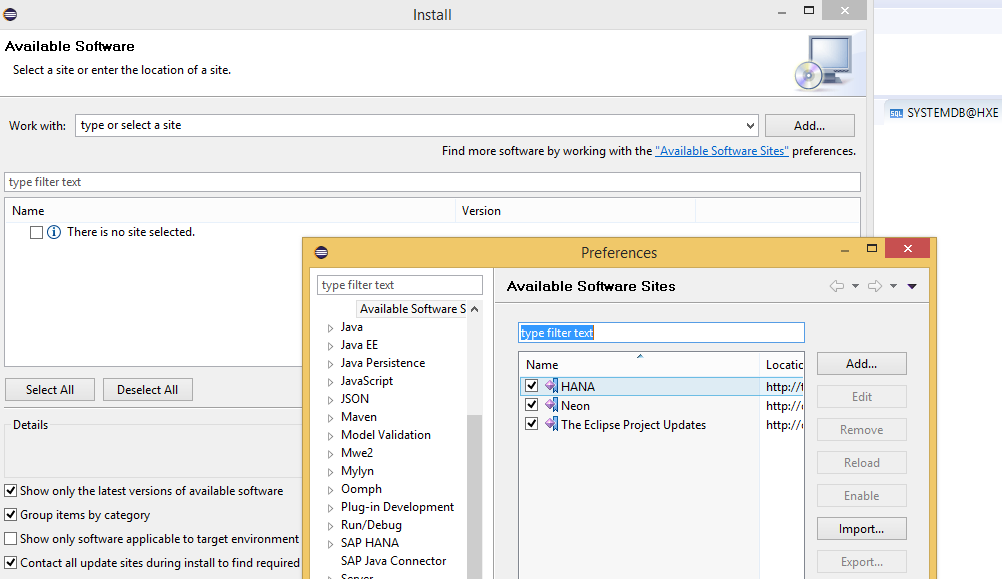
\includegraphics[height=12cm, width=15cm, keepaspectratio]{Hana8.png}
\caption{Eclipse Einstellungen}
\end{figure}    

      \item Sollte der Writer HANA nicht direkt stehen kann man auch auf add gehen und den Link: http://tools.hana.ondemand.com/neon eintragen.

\begin{figure}[H]
\centering
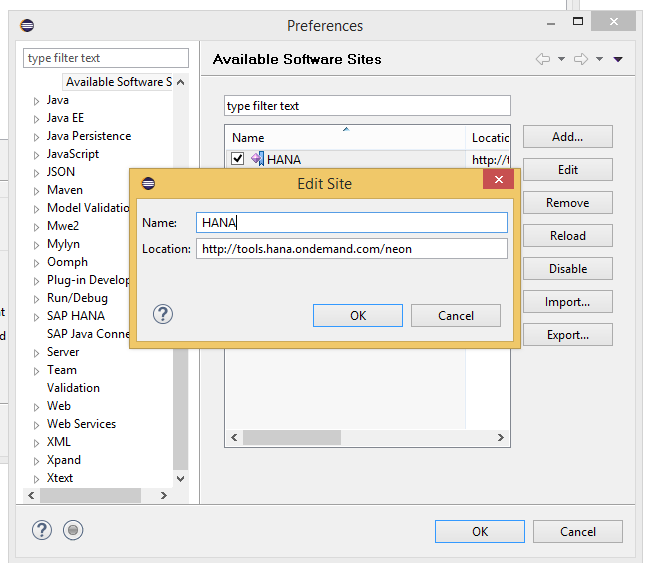
\includegraphics[height=12cm, width=15cm, keepaspectratio]{Hana9.png}
\caption{Eclipse Einstellungen 2}
\end{figure}       


   \end{enumerate}  
  
\end{description}

\subsubsection{Einrichten der Datenbank}
Zunächst wird das System hinzugefügt. 

\begin{figure}[H]
\centering
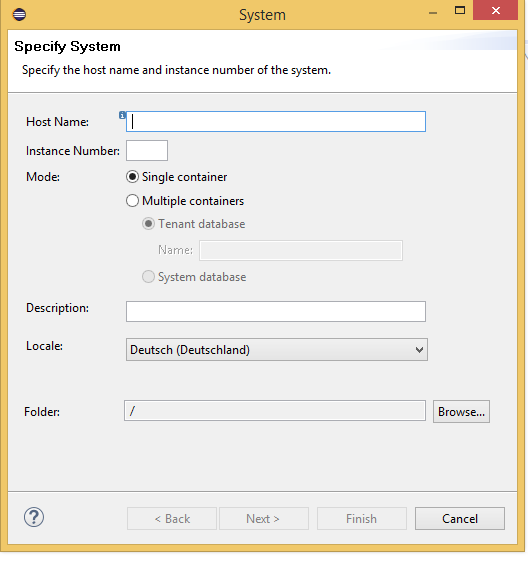
\includegraphics[height=12cm, width=15cm, keepaspectratio]{hanadb1.png}
\caption{System Hinzufügen}
\end{figure}    

      Der Hostname kann unter /sbin/ifconfig gefunden werden.
Die Instanznummer ist standardmäßig 90, für SAP Hana Express 1.0 aber 00.
Mode: Multiple containers -> System database"'. Später noch den Benutzernamen und das festgelegte Passwort angeben sowie einen Hacken bei "`Enable SAP start service connection".

\begin{description}
   \item[Import der Daten]~\par
   \begin{enumerate}
      \item Als erstes unter File auf Import klicken.Es öffnet sich die Importmaske. Wir haben uns die Tabellen als CSV-Dateien auf dem Rechner bereitgelegt und haben daher den Import wisard: Data from Local File verwendet.

\begin{figure}[H]
\centering
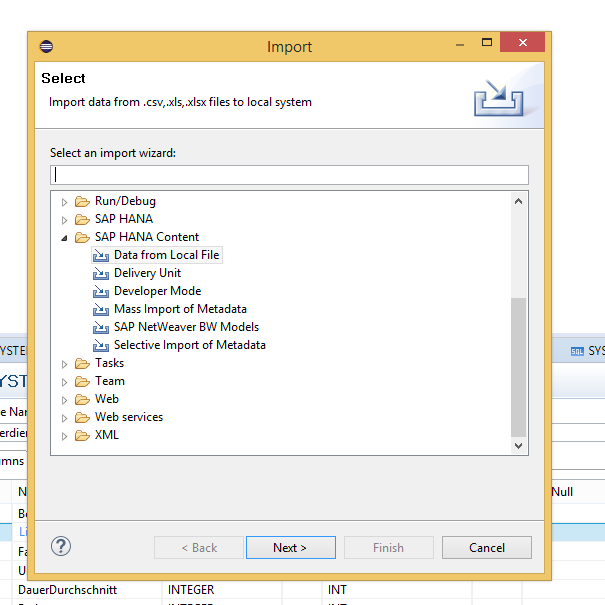
\includegraphics[height=12cm, width=15cm, keepaspectratio]{hanadb2.png}
\caption{Datenimport}
\end{figure}                
		
      \item Als nächstes wählt man die Zieldatenbank aus.

\begin{figure}[H]
\centering
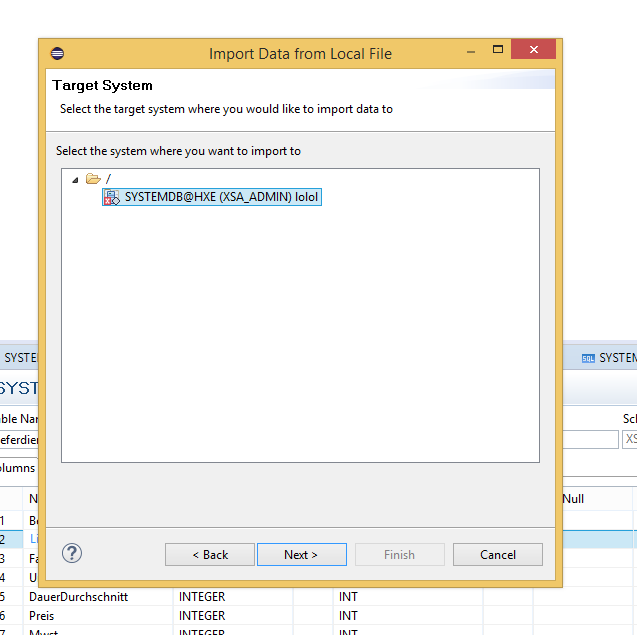
\includegraphics[height=12cm, width=15cm, keepaspectratio]{hanadb3.png}
\caption{Zieldatenbank}
\end{figure}    

      \item Jetzt geben wir den Pfad an, wählen den Delimiter, ob es eine Überschriftenzeile gibt oder nicht sowie das Schema und den Tabellennamen.
      
\begin{figure}[H]
\centering
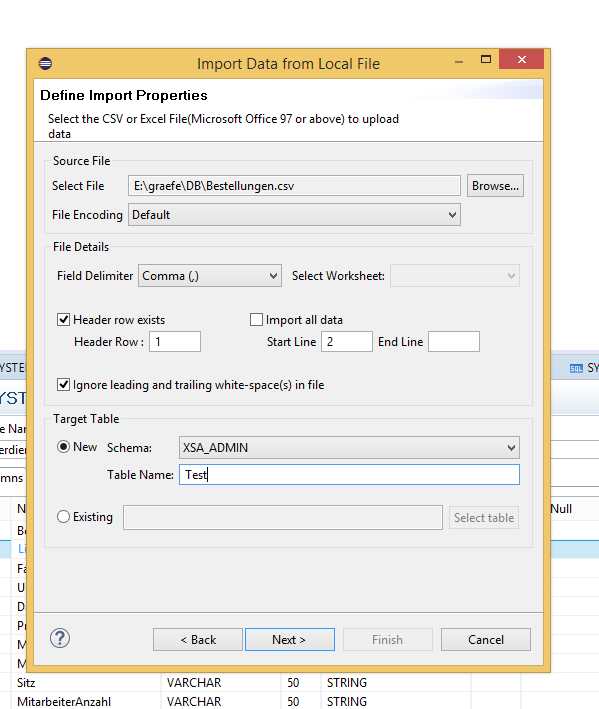
\includegraphics[height=12cm, width=15cm, keepaspectratio]{hanadb4.png}
\caption{Pfadangabe}
\end{figure}          
      
      \item Im nächsten Fenster können wir die Datentypen und die Zuordnung zu der Tabellenstruktur überprüfen und ggf. anpassen. 

\begin{figure}[H]
\centering
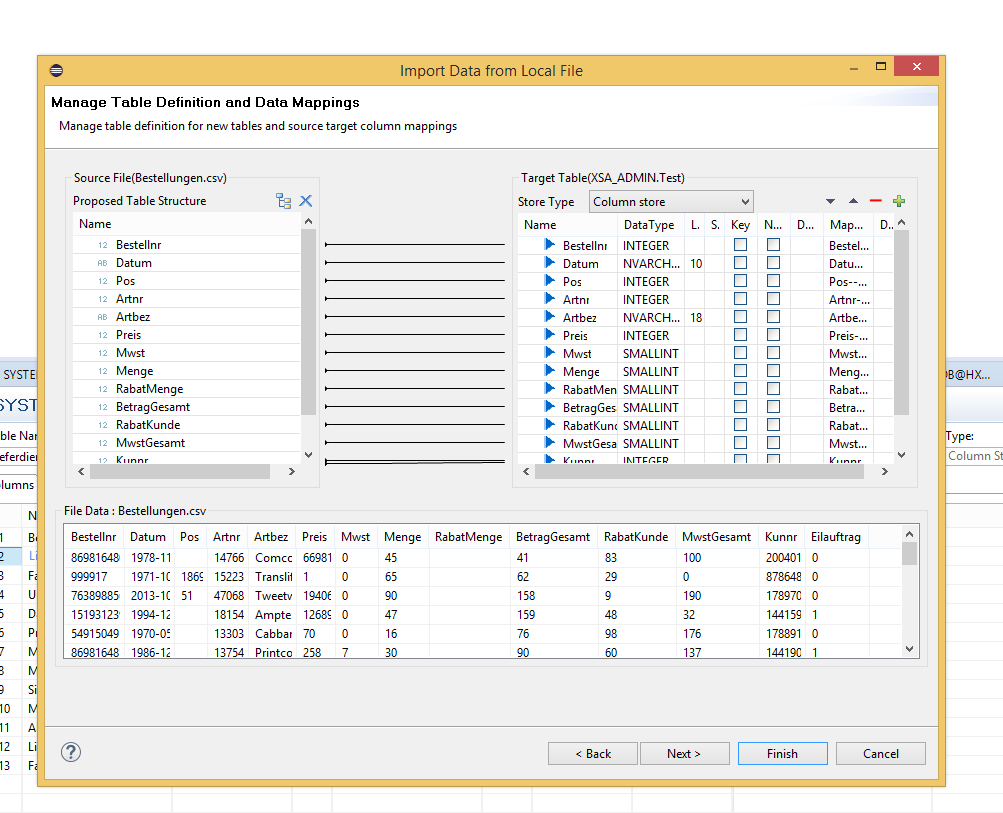
\includegraphics[height=12cm, width=15cm, keepaspectratio]{hanadb5.png}
\caption{Datentypen und Struktur}
\end{figure}    

      \item Als letztes erhält man eine Beispielübersicht auf die importierten Daten.

\begin{figure}[H]
\centering
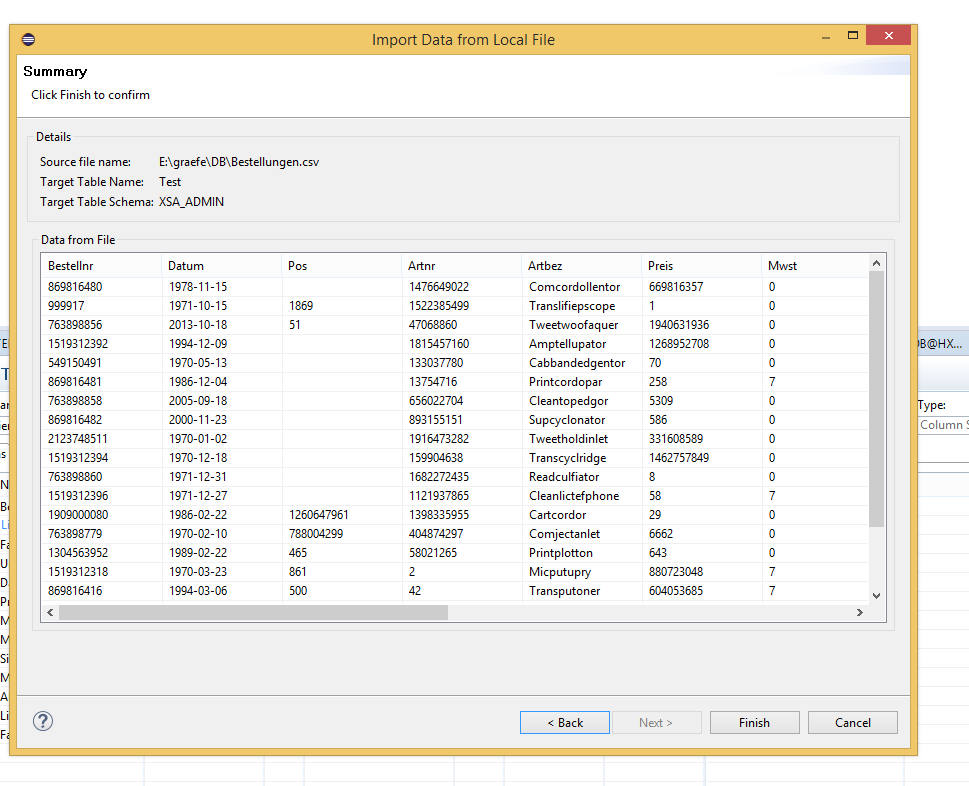
\includegraphics[height=12cm, width=15cm, keepaspectratio]{hanadb6.png}
\caption{Übersicht}
\end{figure}    


   \end{enumerate}  
  
\end{description}






\subsection{Aufsetzen von Cassandra}
\subsubsection{Vorausgehende Schritte}
\begin{description}
   \item[Beschaffung der nötigen Software]~\par
   \begin{enumerate}
      \item Bezogen kann die Installationssoftware für Cassandra von der Apache Foundation. \\http://cassandra.apache.org/download/
      \item Alternativ kann für einen einfachen Windows Installer auch die Version von DataStax Enterprise genutzt werden.\\ https://academy.datastax.com/planet-cassandra/cassandra

   \end{enumerate}  
  
\end{description}

\subsubsection{Installation}
Wir haben uns für den Windows Installer von DataStax entschieden. Die Installation verlief problemlos und man konnte einfach den einzelnen Schritten folgen.
\begin{description}
   \item[Aufsetzen der Cassandra Distribution (DataStax)]~\par
   \begin{enumerate}
      \item Der Installationsumfang besteht dabei aus einer voll funktionstüchtigen Version von Apache Cassandra welche aus einem Server und einer CQL-Shell(Cassandra Query Language) besteht. Zusätzlich gibt es eine Version des DataStax DevCenters die man kostenfrei nutzen kann. 

\begin{figure}[H]
\centering
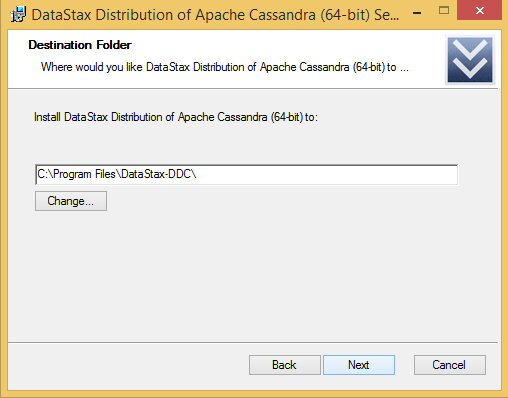
\includegraphics[height=12cm, width=15cm, keepaspectratio]{cass1.png}
\caption{DataStax Zielordner}
\end{figure}    


      \item Nach der erfolgreichen Installation erhält man folgende Verzeichnisstruktur. 

\begin{figure}[H]
\centering
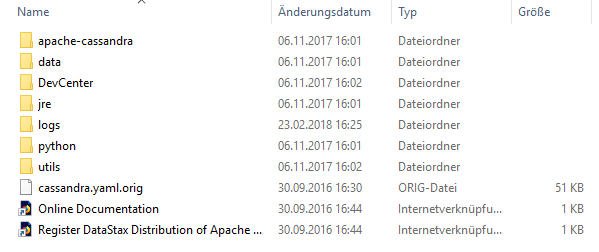
\includegraphics[height=12cm, width=15cm, keepaspectratio]{cass2.png}
\caption{Verzeichnisstruktur}
\end{figure}    


   \end{enumerate}  
  
\end{description}


\begin{description}
   \item[Einrichten von Cassandra]~\par
   \begin{enumerate}
      \item Durch das Ausführen der Cassandra Batch-Datei wird der Server gestartet.
      
\begin{figure}[H]
\centering
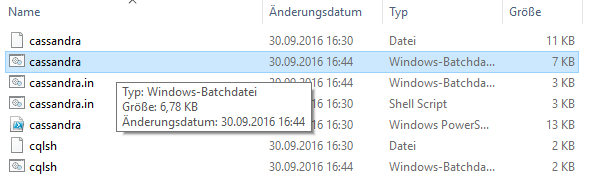
\includegraphics[height=12cm, width=15cm, keepaspectratio]{cass3.png}
\caption{Batch-Datei}
\end{figure}    
       
     
      Dieser Server steht nun zur Verfügung und wartet auf eingehende CQL-Client-Anfragen.
      \item Eine Möglichkeit für einen CQL-Client bietet die in der Installation beinhaltete CQL-Shell die man ebenfalls einfach durch ausführen der „cqlsh.bat“ (Batchdatei) starten kann. Automatisch mit dem Server verbunden, steht diese bereit um Anfragen an den Cassandra-Server zu übertragen. 

\begin{figure}[H]
\centering
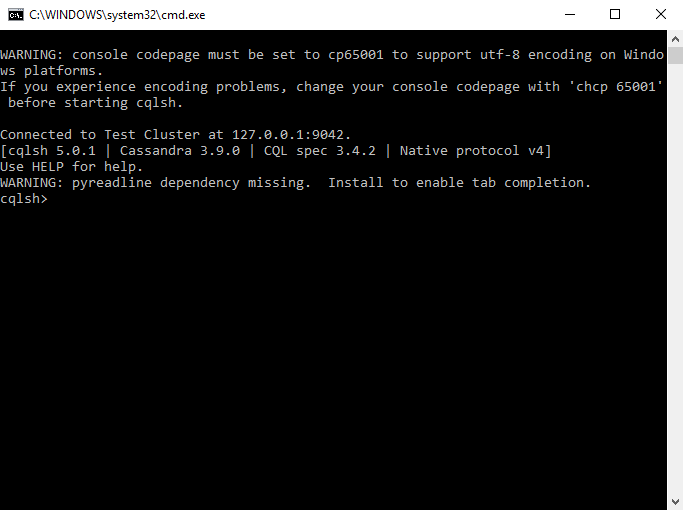
\includegraphics[height=12cm, width=15cm, keepaspectratio]{cass4.png}
\caption{CQL-Client}
\end{figure}    


      \item In der CQL-Shell hat man die Möglichkeit mit Hilfe von CQL-Befehlen mit einer Cassandra-Datenbank zu interagieren.\\

\begin{figure}[H]
\centering
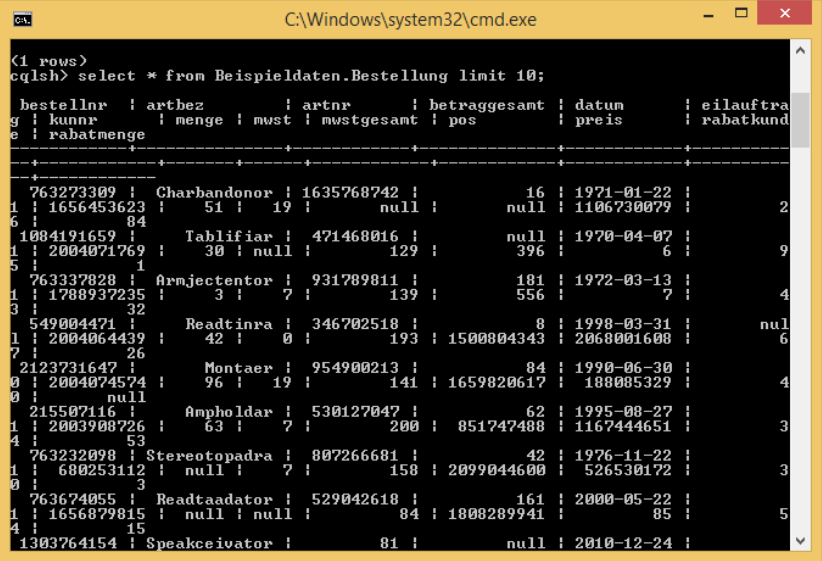
\includegraphics[height=12cm, width=15cm, keepaspectratio]{cass5.png}
\caption{Interaktion}
\end{figure}    

      Wie im Bild zu sehen ist die Übersichtlichkeit in einer Shell stark eingeschränkt zudem gibt es auch einige Probleme mit der Zeichenkodierung. 
      \item Die Vorteile der Cassandra Version von DataStax lagen dabei auch an dem Bereitstellen des DataStax DevCenters. Man hat die Möglichkeit das DevCenter mit dem Server zu verbinden und dieses ebenfalls als CQL-Client zu benutzen um mit der Datenbank arbeiten zu können. Dabei hat man die Vorteile einer übersichtlicheren Oberfläche die keine Probleme mit der Zeichenkodierung hat. 

\begin{figure}[H]
\centering
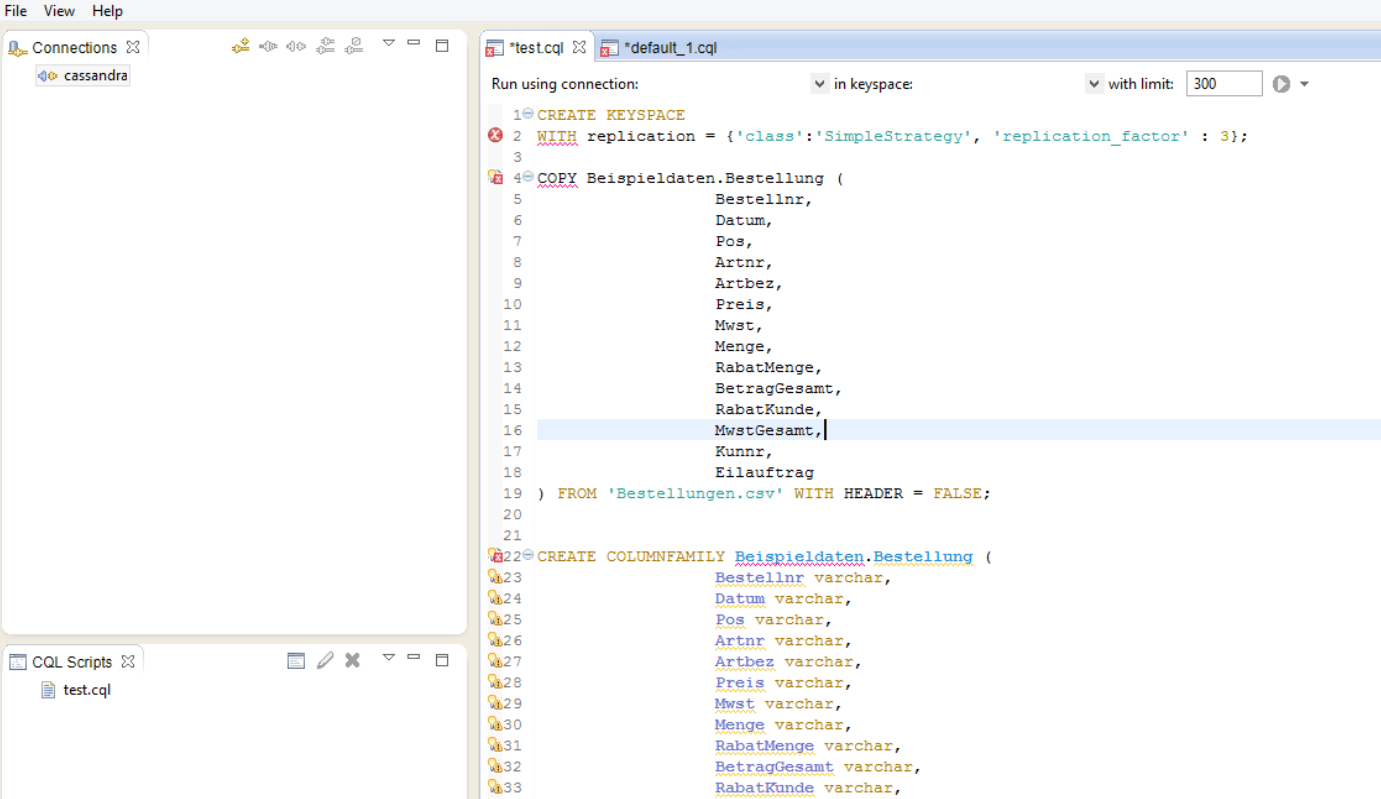
\includegraphics[height=12cm, width=15cm, keepaspectratio]{cass6.png}
\caption{DevCenter}
\end{figure}    


      \item Die Verbindung zwischen dem DevCenter und dem Cassandra-Server stellt man über die Connections-Einstellungen im DevCenter her. \\ Der Server, der auf CQL-Clients im Localhost-Bereich wartet kann über den Port 9042 erreicht werden.

\begin{figure}[H]
\centering
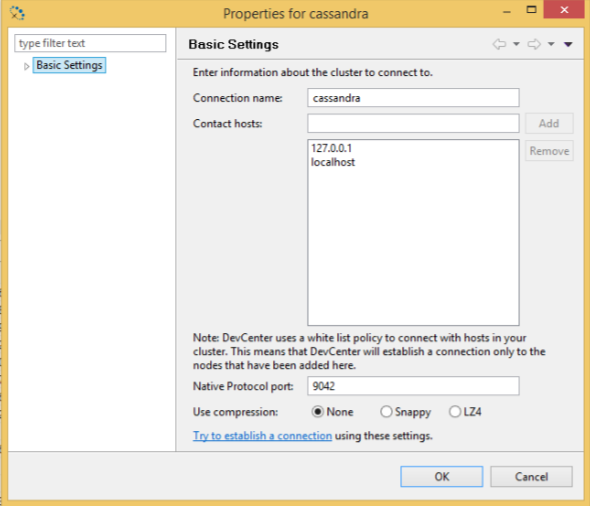
\includegraphics[height=12cm, width=15cm, keepaspectratio]{cass7.png}
\caption{Einstellungen}
\end{figure}    
     

   \end{enumerate}  
  
\end{description}

\subsubsection{Arbeit mit der Cassandra Datenbank}

\begin{description}
   \item[Anlegen der Datenbank]~\par
   \begin{enumerate}
      \item Nachdem das Fallbeispiel in den Systemen von MSSQL und SAPHana aufgesetzt wurde, konnte der Aufbau der Cassandra-Datenbank erfolgen. Als Grundlage dienten hier die von der MSSQL-Datenbank exportierten CSV-Dateien der einzelnen Tabellen. Um die CSV-Dateien erfolgreich importieren zu können, müssen zuerst ein Keyspace und alle Columnfamilies(=Tables) angelegt werden.
      \begin{verbatim}
CREATE KEYSPACE Beispieldaten
WITH replication = {'class':'SimpleStrategy', 'replication_factor' : 1};  	
      \end{verbatim}
		Zu Testzwecken war die „SimpleStrategy“ mit einem "`replication_factor:1"' völlig ausreichend. Die Bedeutung von "`SimpleStrategy"' und "`replication_factor:1"' ist, dass für den einen vorhanden Cassandra-Cluster eine einzelne Replikation als Backup dient.
Es gibt also auch noch die Möglichkeit für jeden weiteren Cluster einen anderen Replikationsfaktor auszuwählen. 

      \item Die Tabellen konnten dann ähnlich wie in SQL einfach mit einem "`CREATE TABLE"' angelegt werden. Hierbei spielt es keine Rolle ob man "`Columnfamily"' oder "`Table"' benutzt.
      \begin{verbatim}
CREATE COLUMNFAMILY Beispieldaten.Kunden (
				  Kunnr varchar,
				  Name varchar,
				  Vorname varchar,
				  PLZ varchar,
				  Ort varchar,
				  Landkz varchar,
				  Land varchar,
				  Bundesland varchar,
				  Region varchar,
				  Debitornr varchar,
				  Kreditorennr varchar,
				  BLZ varchar,
				  IBAN varchar,
				  Kreditinstitut varchar,
				  Beziehungslvl varchar,
				  Werber varchar,
				  PRIMARY KEY(Kunnr));       
      \end{verbatim}
      Der Import der CSV-Dateien erfolgt über den COPY-Befehl.
      \begin{verbatim}
COPY Beispieldaten.Kunden ( 
				  Kunnr,
				  Name,
				  Vorname,
				  PLZ,
				  Ort,
				  Landkz,
				  Land,
				  Bundesland,
				  Region,
				  Debitornr,
				  Kreditorennr,
				  BLZ,
				  IBAN,
				  Kreditinstitut,
				  Beziehungslvl,
				  Werber
) FROM 'KundeUTF.csv' with Header = True; 
      \end{verbatim}		
   \end{enumerate}  
  
\end{description}
Beim Importieren der Daten kam es dann zu ersten Problemen.
Das DataStax DevCenter unterstützt leider nicht die aktuellste Version der CQL(Cassandra Query Language) wodurch der COPY-Befehl nicht ausgeführt werden konnte. Das heißt man muss diesen in der Cassandra-Shell ausführen, welche jedoch auch nach Umstellen der Shell-Eigenschaften bzgl. der Codierung nicht mit den CSV-Dateien umgehen konnte. 
Erst nachdem die CSV-Dateien via Notepad++ in UTF-8 Format gespeichert wurden konnten diese erfolgreich importiert werden.
Der Import erfolgt dann jedoch sehr schnell und dauert trotz 10 Millionen Zeilen lediglich ca. 5 Minuten.







\subsection{Aufsetzen von Maria DB in Kombination mit Memcached}
\subsubsection{Vorausgehende Schritte}
\begin{description}
   \item[Beschaffung der nötigen Software]~\par
   \begin{enumerate}
      \item Download des XAMPP Paketes: \\https://www.apachefriends.org/de/download_success.html
      \item Download PHP-Extension: \\https://github.com/nono303/PHP7-memcache-dll/blob/master/\\vc14/x86/ts/php-7.0.x_memcache.dll
      \item Download Memcached: http://downloads.northscale.com/memcached-win32-1.4.4-14.zip
   \end{enumerate}  
  
\end{description}


\subsubsection{Installationsvorgang}
\begin{description}
   \item[XAMPP installieren]~\par
   \begin{enumerate}
      \item XAMPP wird von www.apachefriends.org heruntergeladen und installiert. Ein Installationsprogramm leitet durch den Installationsprozess und weist bereits auf Typische Probleme mit anderen eventuell installierten Programmen hin. Diese müssen vor der Installation beendet werden.

\begin{figure}[H]
\centering
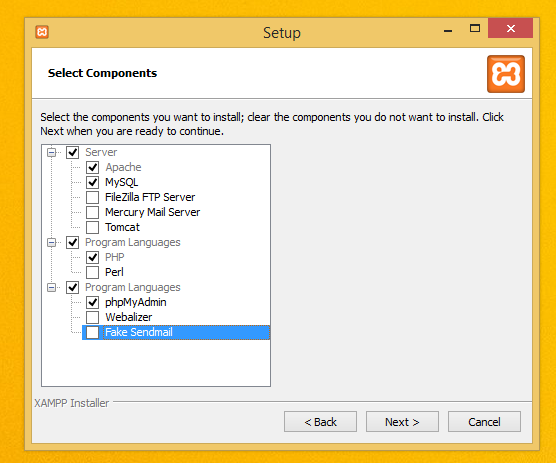
\includegraphics[height=12cm, width=15cm, keepaspectratio]{mem1.png}
\caption{XAMPP Setup}
\end{figure}    


      \item Wichtig ist zu beachten das der Apache-Server auf den Standartports 80 (HTTP) und 443 (SSL) eingerichtet ist und somit keine anderen Prozesse auf dem Rechner laufen dürfen die diese Ports blockieren.

\begin{figure}[H]
\centering
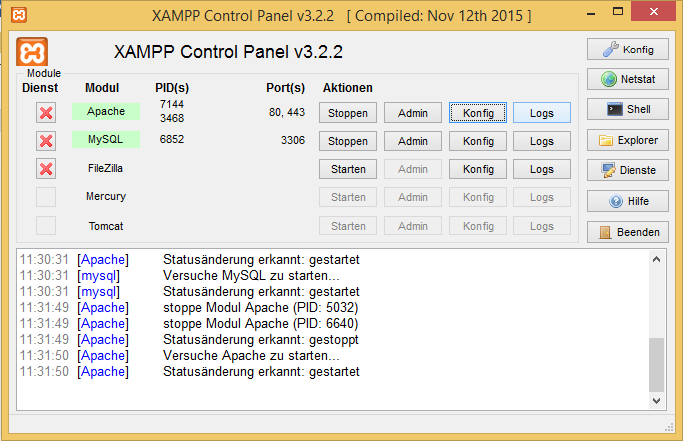
\includegraphics[height=12cm, width=15cm, keepaspectratio]{mem2.png}
\caption{Control Panel}
\end{figure}    


      \item Die Module, wie Apache-Server oder MariaDB können über das im Installationsordner befindliche "`XAMPP Control Panel.exe"' einzeln gestartet und administriert werden.
      Weitere Vorraussetzung ist das der Standartbrowser des Host-Rechners den Zugriff auf die Lokale Domain / IP zulässt.  ("`localhost / 127.0.0.1 "')
      Anschließend ist der Apache-Server nach dem starten über einen beliebigen Browser über die "localhost" Domain/IP erreichbar.	
   \end{enumerate}
   \item[Maria DB einrichten]~\par
   \begin{enumerate}
      \item  Wird in der XAMPP Installation mitgeliefert und ist über den Browser administrierbar (PHPmyAdmin) -- http://localhost/phpmyadmin/
      \item Datenbankstruktur der Testdatenbank wurde über die GUI implementiert 
      \begin{verbatim}
/* Erstellung der 4 Tabellen mit Fremdschlüsseln */
/*Tabelle Kunden anlegen*/
CREATE TABLE Kunden
(Kunnr int Primary Key,
Name varchar(50),
Vorname varchar(50),
PLZ int,
Ort varchar(50),
Landkz varchar(50),
Land varchar(50),
Bundesland varchar(50),
Region varchar(50),
Debitornr int,
Kreditorennr int,
BLZ int,
IBAN int,
Kreditinstitut varchar(50),
Beziehungslvl int,
Werber varchar(50)
)


/*Tabelle Bestellungen anlegen*/
CREATE TABLE Bestellung (
Bestellnr int Primary Key,
Datum date,
Pos int,
Artnr int,
Artbez varchar(50),
Preis int,
Mwst int,
Menge int,
RabattMenge int,
BetragGesamt int,
RabattKunde int,
MwstGesamt int,
Kunnr int,
Eilauftrag int,
Foreign Key (Kunnr) References Kunden(Kunnr)
)
/*Tabelle Lieferdienst anlegen*/
CREATE TABLE Lieferdienst (
Bestellnr int,
Liefernr int Primary Key ,
Fahrzeugtyp varchar(50),
Unternehmen varchar(50),
DauerDurchschnitt int,
Preis int,
Mwst int,
MaxLieferMenge int,
Sitz varchar(50),
MitarbeiterAnzahl int,
Abholstationen int,
Lieferstart int,
Fahrzeuganzahl int,
FOREIGN KEY (Bestellnr) REFERENCES Bestellung(Bestellnr)
)

/*Tabelle Standorte anlegen*/
CREATE TABLE Standorte (
StandortId int Primary Key,
Liefernr int,
Stadt varchar(50),
Landkz varchar(50),
Land varchar(50),
Bundesland varchar(50),
Region varchar(50),
Leitername varchar(50),
Leitervorname varchar(50),
Mitarbeiteranzahl int,
Fuhrparkgröße int,
Gelaendegroeße int,
FOREIGN KEY (Liefernr ) REFERENCES Lieferdienst(Liefernr )

      \end{verbatim}
      
      \item  Zuerst wurde versucht die Daten ebenfalls über die PHPmyAdmin GUI in die Datenbank zu laden. Jedoch begrenzte der Apache-Server die Anzahl der Daten und die Laufzeit der Skripte so stark, das schlussendlich über die mitgelieferte MariaDB Console ein Bulkload der CSV-Dateien erfolgen musste. Diese nahm in etwa 2 Stunden in Anspruch.
      \begin{verbatim}
      /*Bulkload CSV in die Datenbank*/
/*Die Reihenfolge der Füllung ist wegen der FK zu beachten*/

/*1.) Tabelle Kunde laden*/
LOAD DATA LOCAL INFILE 
'C:/Users/stud_admin/Desktop/Gäfe/Tabellen/Kunde.csv'
INTO TABLE kunden FIELDS TERMINATED BY ',' ; 
/*Feldergrenze muss angegeben werden, Rest kann Default bleiben*/

/*2.) Tabelle Bestellungen laden*/
LOAD DATA LOCAL INFILE 
'C:/Users/stud_admin/Desktop/Gäfe/Tabellen/Bestellungen.csv'
INTO TABLE bestellung FIELDS TERMINATED BY ',' ;

/*3.) Tabelle Lieferdienst laden*/
LOAD DATA LOCAL INFILE 
'C:/Users/stud_admin/Desktop/Gäfe/Tabellen/Lieferdienst.csv'
INTO TABLE lieferdienst FIELDS TERMINATED BY ',' ;

/*4.) Tabelle Standorte laden*/
LOAD DATA LOCAL INFILE 
'C:/Users/stud_admin/Desktop/Gäfe/Tabellen/Standorte.csv'
INTO TABLE standorte FIELDS TERMINATED BY ',' ;
      
      \end{verbatim}    
        	
   \end{enumerate}
   \item[Memcache-dll installieren]~\par
   \begin{enumerate}
   	 \item Anschließend muss die .dll in den 
   	 \begin{verbatim}
   	 	php\ext
   	 \end{verbatim} 
   	 Ordner der XAMPP Installation eingefügt werden und über das XAMPP Control Panel in die php.ini in die entsprechende Zeile das "`Extension=memcached.dll"' eingefügt werden.

\begin{figure}[H]
\centering
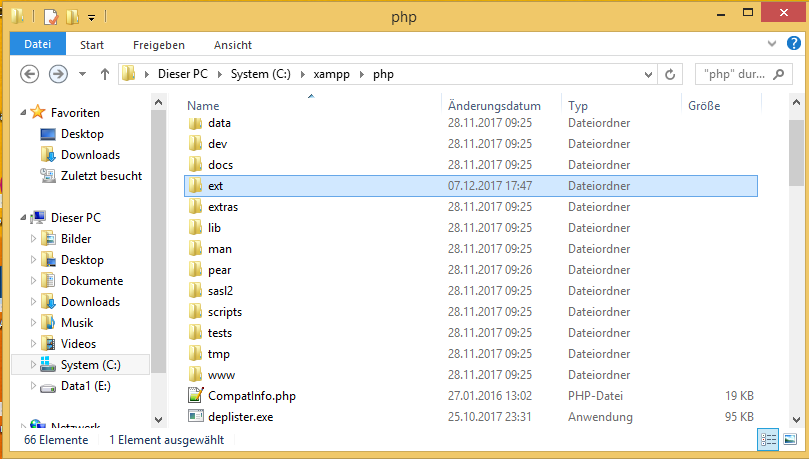
\includegraphics[height=12cm, width=15cm, keepaspectratio]{mem3.png}
\caption{PHP Ordner}
\end{figure} 

\begin{figure}[H]
\centering
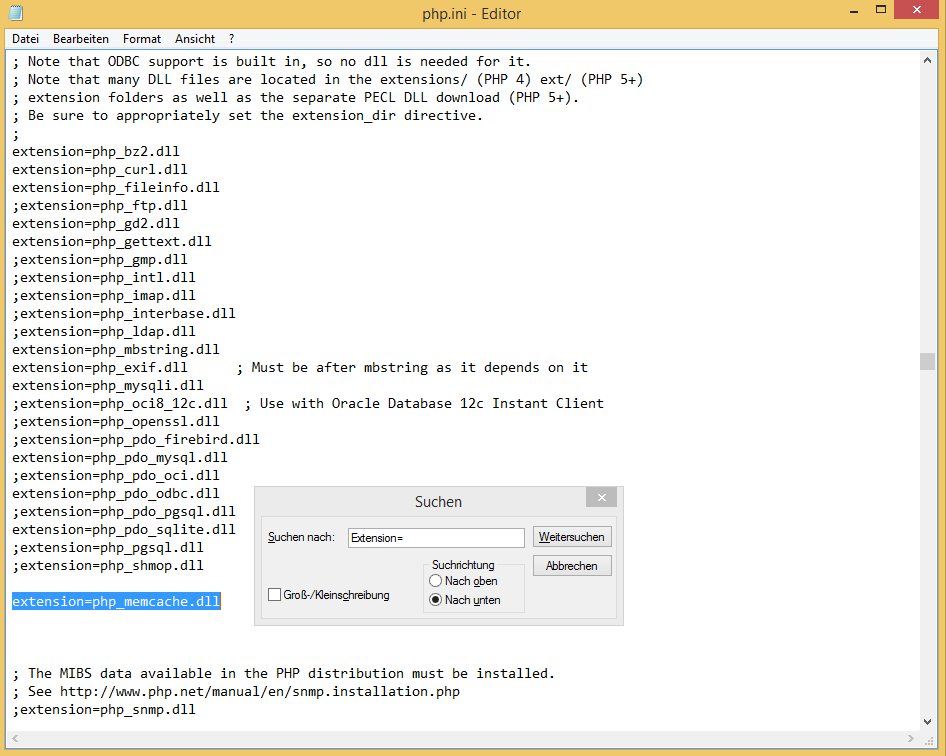
\includegraphics[height=12cm, width=15cm, keepaspectratio]{mem4.png}
\caption{php.ini Datei}
\end{figure} 

   	 Starten der "`php.exe"' im /php Unterordner der XAMPP Installation um
   	 die Extension zu verifizieren und eventuelle Fehlermeldungen zu erhalten. Neustarten des Apache-Servers falls bereits gestartet. Memcached Server sind per default auf dem Port 11211 erreichbar.
   	 \item PHP-Funktionen der Erweiterung
   	 \begin{verbatim}
   	 	$memcached = new Memchached();
$memcached->connect( string $host [, int $port [, int $timeout ]] ) ;

$memcached->set('key', 'value');
$memcached->get('key');

   	 \end{verbatim}
   \end{enumerate}
   \item[Memcached Installation]~\par
   \begin{enumerate}
   		\item Da Memcached ursprünglich für Linux entwickelt wurde sind die meisten Distributionen natürlich für dieses Betriebssystem ausgelegt. Allerdings werden auch Windowsversionen für 32-Bit und 64-Bit Systeme angeboten. Im nachfolgenden wurde die 32-Bit Variante ausgewählt, da unsere Installierte PHP-Engine ebenfalls auf der 32-Bit Architektur basierte.
   		\item Die Installation eines Memcache Servers ist sehr einfach. Das Programm wurde von http://downloads.northscale.com/memcached-1.4.5-x86.zip her-untergeladen und Installiert.
   		\item Dazu einfach die heruntergeladene Ausführbare Datei ausführen und das Programm wird in dem gewählten Ordner installiert
   \end{enumerate}
   
   
\end{description}
\subsubsection{Umsetzung mittels PHP-Engine}
\begin{description}
   \item[Allgemein]~\par
   \begin{enumerate}
   		\item Das von dem Team geschriebene PHP Skript arbeitet nach einem einfachen Prinzip. Es wird eine SQL Abfrage formuliert und über die API wird auf dem Memcache Server geprüft ob diese Abfrage in letzter Zeit bereits getätigt wurde. Dazu wird die Abfrage mit den Keys des Memcache Servers verglichen. Sollte diese Abfrage noch nicht gestellt worden und damit im Memcache Server abgelegt worden sein, wird eine reguläre Abfrage an die MariaDB gestellt. Dabei wird direkt vor und nach dem Abfragen die System-zeit aufgenommen und nachher die Differenz berechnet. Anschließend wird in diesem Fall die Abfrage als Key und das Ergebnis als Value auf dem Memcache Server abgelegt. Somit kann das Ergebnis bei erneuter Abfrage direkt aus dem Memcache geladen werden.
   		\item Die Vorgehensweise zum Ermitteln der Abfragedauern erfolgte folgender-weise. Es wurden 5 Abfragen an die SQL DB gestellt und deren Abfrage dauern aufgenommen. Anschließend wurde diese Abfrage wiederholt, in das Memcache gespeichert und der Value des Memcache Servers 5 mal abgefragt. Auch hier wurde die Zeit erneut nach demselben Prinzip aufgenommen. Zum Schluss wurden die Ergebnisse der beiden Versuche verglichen.


   \end{enumerate}
   \newpage
   \item[Ablauf]~\par 
   \begin{enumerate}
   		\item Abfrage->(Zeitstempel)Check ob in Memcache Vorhanden -> Ja –(Zeitstempel und Differenz errechnen)> Ausgeben
   		\item Abfrage -> Check ob in Memcache Vorhanden -> Nein ->(Zeitstempel) Aus DB holen (Zeitstempel und Differenz errechnen) -> in Memcache speichern -> Ausgeben
   		\item Verwendetes PHP-Skript und HTML-Code
   		\begin{verbatim}
<!DOCTYPE html>
<html lang="de">
 <head>
 <meta charset="utf-8">
 <meta http-equiv="X-UA-Compatible" content="IE=edge">
 <meta name="viewport" content="width=device-width, initial-scale=1">
 <title>Projektseminar</title>
 <link href="data/css/style.css" rel="stylesheet">
 <style>
 table, th, td {
 border: 1px solid black;
 }
 </style>
 
 
 </head>
 <body style="background-image: url('bg.jpg');">
 <div class="page-header">
		<h1>Projektseminar<br><small></small></h1>
  </div>
<?php
include ("C:\Users\\robin\Desktop\HTML_Schmiede\htdocs\Projektseminar\data\php\config.php");
//Initialisiere Handle Klassen
$mysql = new MySQL_DB();
$memcached = new Memcached();
$print = new print_result();


//Verbinde zu Servern | Einstellungen in config.php
$mysql->connect();
$memcached->connect();

//Input SQL Abfrage:
$sql="SELECT * FROM accounts WHERE acc_name= 'test' AND acc_pw = 123";
//$sql="SELECT * FROM `provinces`";



//Suche im Memcached
$beginn = microtime(true); // Nimm die Systemzeit vor abfrage
	if($mem_result=$memcached->get($sql)){	
		$dauer = (microtime(true)-$beginn)*1000;
		//Wenn gefunden -> Ausgabe	
		echo "Im Memcached gefunden!<br><br>";
		echo"<br>Abfragedauer Memcached: $dauer ms<br>";		
		
		//Ausgabe
			
			//Als Text
			//print_r($mem_result);
		
			//Ausgabe als Tabelle
			//$print->print_table($mem_result);		

		
		}
		//Wenn nicht:
			else{
			echo "Nicht im Memcached gefunden.<br>";
			echo "Aus der Datenbank geholt.<br>";
			//DB anrufen und fragen
			$result=$mysql->query($sql);
			
			//Ergebnisse ausgeben
				
				//Als Text
				//print_r($result);

				//Ausgabe als Tabelle		
				//$print->print_table($result);

			
			echo "Anzahl der Zeilen: " . count($result);
			
			
			//Ergebnisse im Memcached ablegen
			$memcached->set($sql,$result);
			}
	//Werte dauer des Vorgangs aus

	

?>

  </body>
</html>

   		\end{verbatim}
   \end{enumerate}
\end{description}
  
   


\newpage
\section{Vergleichender Performancetest}
\subsection{Vergleich insgesamt}
Hier der quantitative Vergleich der Datenbanksysteme im Allgemeinen:\\
Es wurde die verstrichene Zeit vom Bestätigen der Query durch den User bis hin zu Anzeige des Ergebnisses im GUI je System zehn Mal gemessen und daraus ein Durchschnitt gebildet worden.

\begin{figure}[H]
\centering
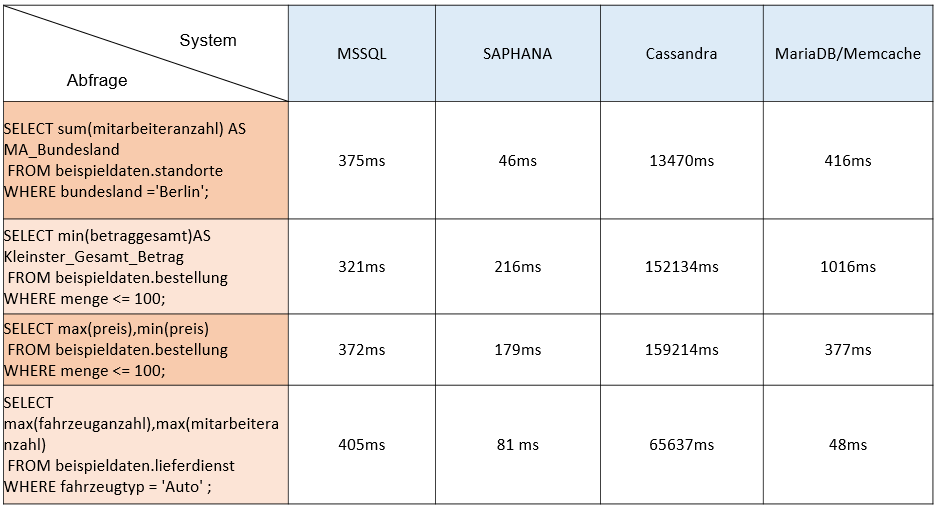
\includegraphics[height=12cm, width=15cm, keepaspectratio]{ausw1.png}
\caption{Übersicht Systeme}
\end{figure}  

Insgesamt stellt sich SAP Hana Express als schnellstes DB-System heraus. Cassandra ist am Langsamsten und Maria DB/ Memcache variiert in der Leistung. MSSQL stellt sich als zweitschnellstes System heraus.
Diese Abfragen haben wir extra für den Vergleich aller Systeme gewählt. Cassandra und Memcache konnten ab einer gewissen Größe der zu der analysierenden Datenmenge keine Ergebnisse mehr anzeigen. 
Das Arbeiten in der Shell führte dann aber zu dem Problem, dass es keine Möglichkeit gab die Zeiten pro Abfrage zu sehen bzw. anzeigen zu lassen.
Folglich musste via CAPTURE-Befehl eine Textdatei angegeben werden, in der eine detaillierte Anzeige des Outputs samt Zeiten aufgelistet wird.
\begin{verbatim}
CAPTURE 'Logdatei.txt‘ ON
\end{verbatim}

Leider führte das Anlegen der Logdateien zu leichten Verfälschungen bei den Abfragezeiten was den allgemeinen Vergleich jedoch nicht weiter beeinträchtigte, da Cassandra von den Zeiten her , sowieso um Längen geschlagen wird.
\subsection{SAP Hana Express im Quantitativen Vergleich zu MSSQL}
Hier sechs Vergleichs-Abfragen von SAP Hana und MSSQL. Es wurden  sechs Querys getestet. 
\begin{description}
	\item[Diese wurde falls möglich zehn Mal wiederholt:]~\par 
	\begin{enumerate}
		\item Abfrage: 
		\begin{verbatim}
Select k."Name", k."Vorname", k."Kreditorennr", k."Land", 
b."Artbez", b."BetragGesamt", b."Menge", b."MwstGesamt", b."RabatMenge", 
l."Abholstationen", l."DauerDurchschnitt", l."Unternehmen",
s."Leitername", s."Leitervorname"
From "XSA_ADMIN"."Kunde" k 
Inner Join "XSA_ADMIN"."Bestellung" b On (k."Kunnr" = b."Kunnr")
Inner Join "XSA_ADMIN"."Lieferdienst" l On (b."Bestellnr" = l."Bestellnr")
Inner Join "XSA_ADMIN"."Standorte" s On (l."Liefernr" = s."Liefernr")
Order by k."Name"; 
		\end{verbatim}
		\item Abfrage: 
		\begin{verbatim}
Select k."Name", k."Vorname", k."Kreditorennr", k."Land", 
b."Artbez", b."BetragGesamt", b."Menge", b."MwstGesamt", b."RabatMenge", 
(b."Menge" * b."BetragGesamt") As SumRand,
(b."BetragGesamt" * b."MwstGesamt" - ((b."Menge" - b."RabatMenge")/100) * b."BetragGesamt") As test,
l."Abholstationen", l."DauerDurchschnitt", l."Unternehmen",
s."Leitername", s."Leitervorname"
From "XSA_ADMIN"."Kunde" k 
Inner Join "XSA_ADMIN"."Bestellung" b On (k."Kunnr" = b."Kunnr")
Inner Join "XSA_ADMIN"."Lieferdienst" l On (b."Bestellnr" = l."Bestellnr")
Inner Join "XSA_ADMIN"."Standorte" s On (l."Liefernr" = s."Liefernr")
Order by k."Name";
		\end{verbatim}
		\item Abfrage: 
		\begin{verbatim}
SELECT AVG (cast (a."Preis" as bigint)) AS AVGLief, AVG (cast(b."Preis" as bigint)) AS AVGBestell, AVG (cast (c."Mitarbeiteranzahl" as bigint)) AS AVGMit 
 FROM "XSA_ADMIN"."Lieferdienst" a, "XSA_ADMIN"."Bestellung" b, "XSA_ADMIN"."Standorte" c
 WHERE c."Liefernr" = a."Liefernr" AND b."Bestellnr" = a."Bestellnr"
GROUP BY a."Preis";
		\end{verbatim}
		\begin{enumerate}
			\item Abfrage:
			\begin{verbatim}
SELECT AVG (cast (a."Preis" as bigint))/(SELECT SUM(cast("Preis" as bigint)) FROM "XSA_ADMIN"."Bestellung") * (SELECT AVG(cast("Preis" as bigint)) FROM "XSA_ADMIN"."Bestellung")   AS AVGLief, AVG (cast(b."Preis" as bigint)) AS AVGBestell, AVG (cast (c."Mitarbeiteranzahl" as bigint)) AS AVGMit 
 FROM "XSA_ADMIN"."Lieferdienst" a, "XSA_ADMIN"."Bestellung" b, "XSA_ADMIN"."Standorte" c
 WHERE c."Liefernr" = a."Liefernr" AND b."Bestellnr" = a."Bestellnr"
GROUP BY a."Preis";
			\end{verbatim}
		\end{enumerate}
		\item Abfrage:
		\begin{verbatim}
SELECT sum(cast(s."Fuhrparkgröße" as bigint)) AS "SummeFuhrparkgröße", b."Datum"
 FROM "XSA_ADMIN"."Bestellung" b , "XSA_ADMIN"."Standorte" s
 Where b."Datum" = '2003-07-08'
GROUP BY "Datum"; 
		\end{verbatim}
		\item Abfrage: 
		\begin{verbatim}
Select AVG ("RabatKunde") AS DurchschnittlicherRabattKunde, k."Name", l."Liefernr"
 FROM "XSA_ADMIN"."Lieferdienst" l , "XSA_ADMIN"."Kunde" k Join "XSA_ADMIN"."Bestellung" b ON (k."Kunnr" = b."Kunnr") 
Group By k."Name", l."Liefernr";
		\end{verbatim}
		\item Abfrage: 
		\begin{verbatim}
Select AVG (cast (l."Bestellnr" as bigint)) As AVGBestellProLief, l."Unternehmen"
FROM "XSA_ADMIN"."Bestellung" b 
JOIN "XSA_ADMIN"."Lieferdienst" l ON(b."Bestellnr" = l."Bestellnr")
Group BY l."Unternehmen"; 
		\end{verbatim}
		
		
	\end{enumerate}
\end{description}
Dabei konnte SAP Hana Express bei Abfrage 1, 2 und 5 kein vollständiges Ergebnis ausgeben. 
Wir vermuten, dass der Arbeitsspeicher voll ausgelastet war und keine Weiteren Ergebnisse mehr dort gespeichert werden konnten ehe alte Daten gelöscht wurden.
Als wir uns bei den Kritischen Abfragen über den Taskmanager die Ressourcenauslastung des PCs haben anzeigen lassen, bestätigte dies die Theorie. Der Arbeitsspeicher war komplett ausgelastet.
Da man SAP Hana Express nur maximal 30 GB Arbeitsspeicher zuweisen kann, haben wir also die Grenze von SAP Hana Express ausgelotet.
Sobald die Anzahl der Ergebnisdatensätze zu hoch wird kann SAP Hana Express die Abfrage nicht mehr zuverlässig und schnell bearbeiten.
Die Ergebnisse der durchführbaren Abfragen haben wir in Diagrammen zusammengetragen:

\begin{figure}[H]
\centering
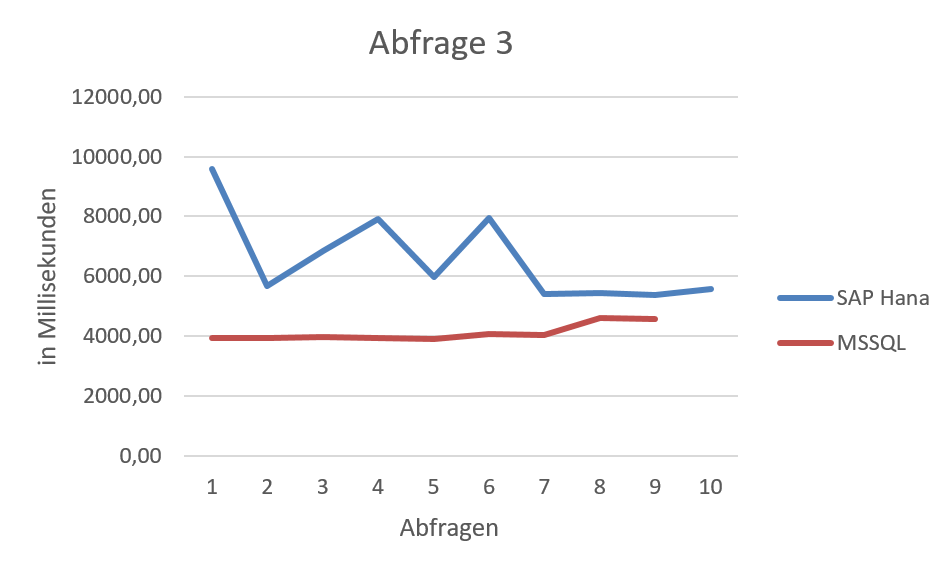
\includegraphics[height=12cm, width=15cm, keepaspectratio]{diag1.png}
\caption{Abfrage 3}
\end{figure}  

\begin{figure}[H]
\centering
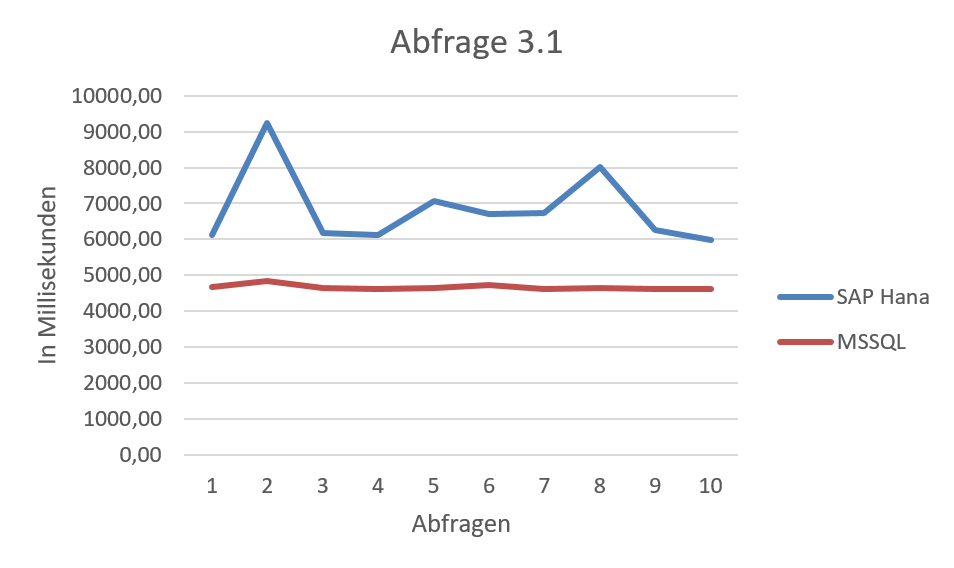
\includegraphics[height=12cm, width=15cm, keepaspectratio]{diag2.png}
\caption{Abfrage 3.1}
\end{figure}  

\begin{figure}[H]
\centering
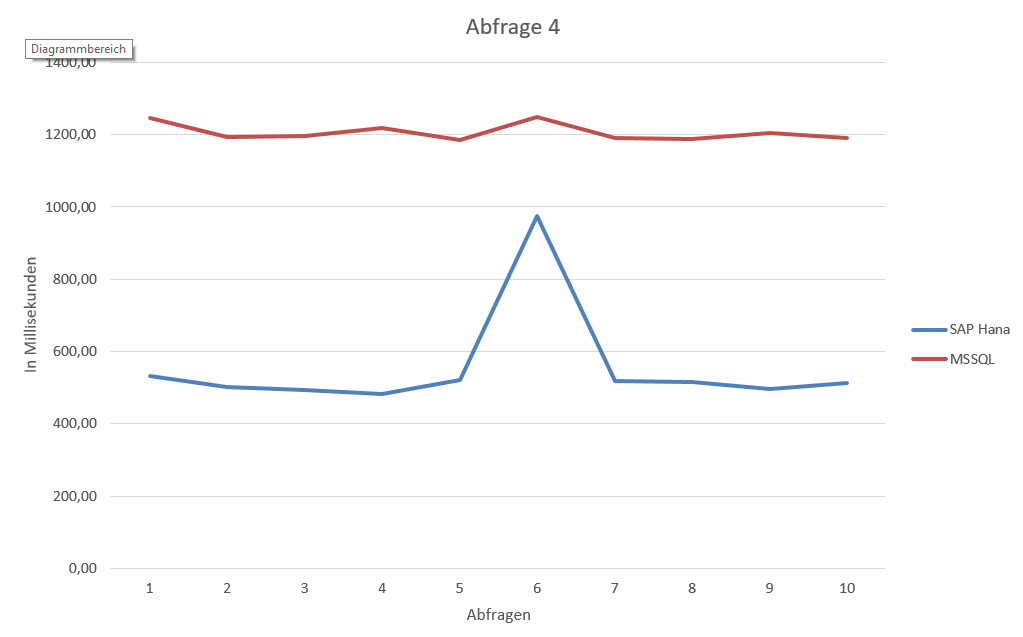
\includegraphics[height=12cm, width=15cm, keepaspectratio]{diag3.png}
\caption{Abfrage 4}
\end{figure}  

\begin{figure}[H]
\centering
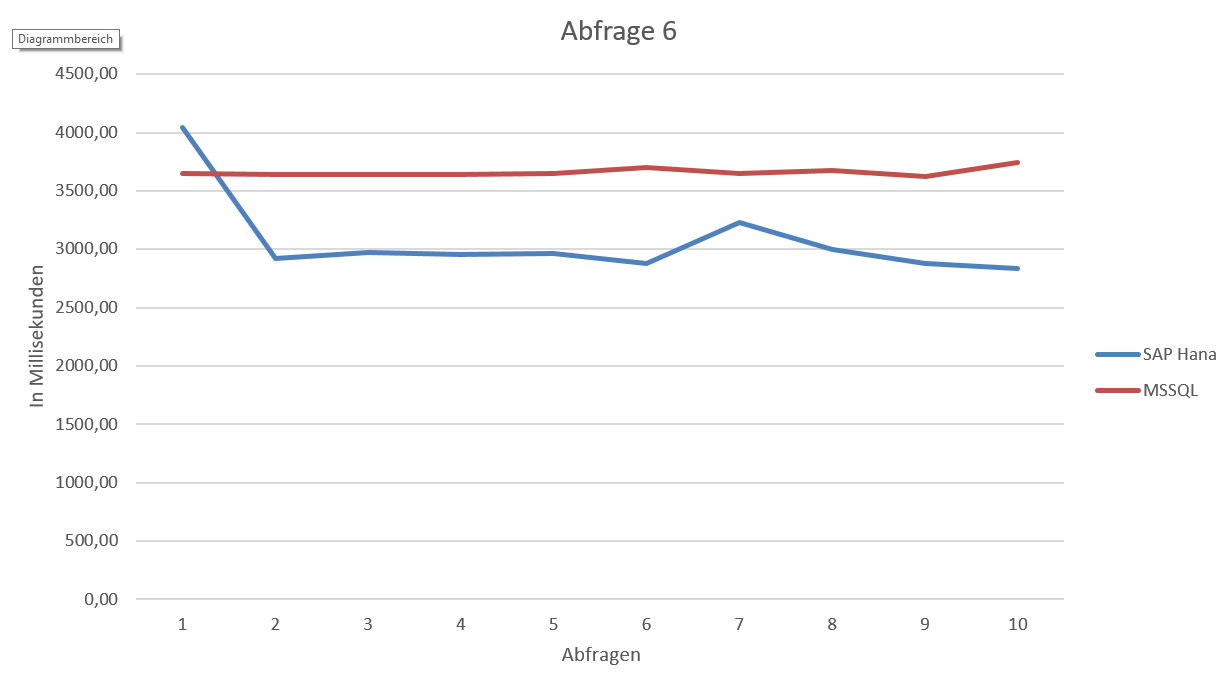
\includegraphics[height=12cm, width=15cm, keepaspectratio]{diag4.png}
\caption{Abfrage 6}
\end{figure}  

Bei sehr komplexen Abfragen kann nur noch MSSQL Server 2016 zuverlässig Ergebnisse liefern. Aber selbst bei solch komplexen Abfragen kann SAP Hana Express teilweise durch schnellere Abfragezeiten glänzen. 
Grade bei Abfrage 6 und Abfrage 3 kann man die Vorteile von SAP Hana Express sehen. Es wird wie bei den anderen In-Memory-DB-Systemen Logdateien der Abfragen erstellt, um die Verfügbarkeit nach einem Absturz des PCs sicherzustellen. SAP Hana Express kann diese Logdateien dazu nutzen seine Performance noch weiter zu optimieren in dem es auf diese Logdateien zugreift und damit die Abfrage löst. Somit werden bei wiederholter Durchführung der gleichen Abfrage die Antwortzeiten des Programmes noch weiter verringert.
\subsection{Qualitativer Vergleich der DB-Systeme}
\subsubsection{SAP Hana Express:}
\subsubsection{Vorteile}
SAP Hana Express bietet gute und vielfältige Komprimierungsverfahren und bietet dem Nutzer die angewendeten Verfahren zu bestimmen oder zu verändern. Somit lässt es sich besser auf die direkte Aufgabe des DB-Systems im Anwendungsfall einstellen.
Durch die Nutzung von Eclipse war das GUI von SAP Hana Express relativ intuitiv und man konnte sich schnell zurechtfinden. Es ist nah an die GUI von ähnlichen Programmen angelegt.
Ein Pluspunkt ist natürlich auch, dass SAP Hana Express kostenlos zur Verfügung gestellt wird.

\subsubsection{Nachteile}
Es gibt nur eine Linux Version des Programms und man ist als Windows-Nutzer dazu gezwungen eine VM zu nutzen.
Die Express-Version von SAP Hana deckt nur eine Nutzung von maximal 32 GB Arbeitsspeicher ab.
Die Syntax ist komplizierter und "`unhandlicher"' gestaltet als die vergleichbarer Programme. So müssen Felder und Spaltennamen immer mit Anführungszeichen angegeben werden und die genutzte Datenbank muss jedes Mal aufgeführt werden.

\subsubsection{MSSQL Server 2016:}
\subsubsection{Vorteile:}
Die bekannte Oberfläche sowie die gewohnte einfache Syntax von MSSQL tragen zu einer komfortablen und intuitiven Bedienung bei.
Beim Erstellen der Abfragen kam uns MSSQL Server 2016 am meisten mit seiner Robusten Fehlerhilfe, den vielen vorgefertigten Funktionen und ähnlichen Hilfen sehr entgegen.
Insgesamt ist MSSQL ein guter Allrounder das eine breite Auswahl an Hilfsmitteln und Tools bereitstellt.

\subsubsection{Nachteile: }
Im Vergleich zu SAP Hana Express war keine Einflussnahme des Nutzers auf die Komprimierung möglich und auch sonst hielt sich Microsoft auch mit Hintergrundinformationen zurück.
Einschränkungen zu Aufrechterhaltung der referentiellen Integrität konnten nicht auf In-Memory-Datenbanken angewendet werden, so wurden Check, Foreign Key und Unique nicht unterstützt.

\subsubsection{Cassandra}
\subsubsection{Vorteile:}
Eine Horizontale Skalierbarkeit der Hardware Ressourcen ermöglicht einen Einsatz von Cassandra unabhängig von der Größe der Daten.
Cassandra setzt auf eine Vermeidung unnötiger Komplexität sowie die Vermeidung von relationalen Ansätzen des Datenmappings. 
Eine Replikation der Datenbank ist sehr einfach möglich.
Es handelt sich um eine kostenlose Open Source Software.

\subsubsection{Nachteile:}
Ein Mangel an umfangreichen Dokumentationen machte die Arbeit mit Cassandra eher schwierig. 
Es handelt sich nicht um eine universelle Sprache wie SQL.
Teilweise unerwartetes Verhalten und fehlender Support erschweren den Umgang mit der Software.


\subsubsection{Memcache}
\subsubsection{Vorteile}
Eine sehr einfache Installation sowie Implementation machen Memcache auch für Einsteiger gut Nutzbar.
Auch in der Bedienung ist Memcache sehr einfach und zeichnet sich durch simple Befehle wie:
Set(), add() und get() aus.
Es handelt sich um eine kostenlose Open Source Software.

\subsubsection{Nachteile}
Bei Open Source können auch immer Fehler im Code ausgenutzt werden.
Überhaupt wird die Sicherheit komplett dem Nutzer überlassen und kann daher zu Fatalen Sicherheitslücken führen.
Die Kompression ist von den genutzten Bibliotheken und Programmiersprachen abhängig, weshalb ein Wechsel dieser innerhalb der Datenbank nicht unterstützt wird und Fehlfunktionen auslösen kann.

\newpage
\section{Systemvergleich}
\subsection{SAP Hana Express}
\begin{description}
	\item[Vorteile]~\par
	\begin{itemize}
		\item Haltung der kompletten Datenbank im Hauptspeicher. 
		\item Gute Komprimierungsverfahren ermöglichen Anwendung auch bei sehr großen Datenbanken. 

		\item Ein schneller Zugriff.

		\item Grundlage für OLTP und OLAP.
		
	\end{itemize}
\end{description}


\begin{description}
	\item[Nachteile]~\par
	\begin{itemize}
		\item Kompliziertere Benutzeroberfläche (grade bei Express Version).

		\item Nur Linux Version.
		\item Einschränkungen der Komprimierungsverfahren durch teilweise nicht mehr direkten Zugriff auf Daten.
		\item Viele Verfahren zur Komprimierung benötigen Sortierung die nur nach einer Tabellenspalte geht.

		\item Hohe Speicherkosten und Speicher als neuer Bottleneck.

		\item Hohe Kosten für Produkt (SAP Hana). Und Aufpreise bei Erweiterung der Express Version. 
	\end{itemize}
\end{description}

\subsection{MS SQL Server}
\begin{description}
	\item[Vorteile]~\par
	\begin{itemize}
		\item Schnellerer Zugriff auf Tabellen da Datenhaltung derer IN Arbeitsspeicher (geringe Latenz).

		\item Multiversionsverwaltung (mehrere Datensätze in einer Transaktion -> jede davon nutzt eigene Version der Datensätze) 

		\item Keine Komprimierung zwingend Notwendig da nur einzelne Tabellen in Speicher gehalten werden. 

		\item Gewohnte Oberfläche durch Zugriff und Arbeit mit SQL Server Management Studio.
		
	\end{itemize}
\end{description}


\begin{description}
	\item[Nachteile]~\par
	\begin{itemize}
		\item Einschränkungen -> Check, Foreign Key, Unique beispielsweise erst nicht unterstützt.
		\item Da keine Komprimierung erfolgt nur begrenzte Nutzbarkeit bei sehr großen Datenbanken (dann wird auch sehr viel Arbeitsspeicher benötigt).
		\item Wesentlich höhere Kosten für Hauptspeicher, trotzdem ist dieser noch Bottleneck



	\end{itemize}
\end{description}

\subsection{Cassandra}

\begin{description}
	\item[Vorteile]~\par
	\begin{itemize}
		\item Möglichkeit der horizontale Skalierbarkeit.
		\item Vermeiden unnötiger Komplexität.
		\item Bietet hohe Performance und hohen Durchsatz.
		\item Vermeidung von relationalen Ansätzen des Datenmappings.
		\item Einfachere Replikation der Datenbanken. 

	\end{itemize}
\end{description}


\begin{description}
	\item[Nachteile]~\par
	\begin{itemize}
		\item Mangel an umfangreichen Dokumentationen. 
		\item Keine universelle Sprache wie SQL. 
		\item Unerwartetes Verhalten und fehlender Support. 
		
	\end{itemize}
\end{description}

\subsection{Maria DB mit Memcache}

\begin{description}
	\item[Vorteile]~\par
	\begin{itemize}
		\item Einfach zu installieren und implementieren.
		\item Einfache Optimierung der Ladezeiten von Webseiten.
		\item einfache Bedienung durch z.B.: 
		\begin{verbatim}
			set() ; add() ; get()  
		\end{verbatim} 
		\item Open Source (BSD-Lizenz).


	\end{itemize}
\end{description}


\begin{description}
	\item[Nachteile]~\par
	\begin{itemize}
		\item Open Source, dadurch sind Fehler im Code ausnutzbar.
		\item Sicherheit außerdem fast vollständig vom Nutzer / Bibliothek abhängig. 
		\item Kompression von Bibliothek / Programmiersprache abhängig. 
		\item Memcache sollte nur von einer Bibliothek angesprochen werden (Unterschiedliche Arten der Abspeicherung von Daten / Kompressionsmethoden).

	\end{itemize}
\end{description}

\newpage
\section{Fazit}
Ein Semester haben wir uns intensiv mit den verschiedenen Systemen auseinandergesetzt. Dabei sind wir leider auch immer wieder auf Probleme gestoßen. Am wenigstens gab es diese bei dem MS SQL Server. Er lies sich sehr leicht installieren und wie gewohnt bedienen. Bei SAP Hana Express gab es einige Probleme während der Installation, weshalb der Prozess mehrmals von neuem begonnen werden musste. Die Umgebung erwies sich hier teilweise als Übeltäter. So mussten noch mehrere Konfigurationen vorgenommen werden. Cassandra machte zunächst Schwierigkeiten beim einfügen der Daten die wir generiert haben. Zunächst konnte man im DevCenter von DataStax dem COPY- Befehl nicht ausführen. Der Datenimport musste also in der Cassandra-Shell ausgeführt werden, die wiederum nicht mit den CSV Dateien umgehen konnte. Diese haben wir dann noch in das UTF-8 Format gebracht (mit Hilfe von Notepad++). Nachdem wir Probleme wie diese gelöst hatten, konnten wird aber mit allen Systemen gut arbeiten. Wobei sich diese sich sehr unterscheiden.\\
SAP HANA Express eignet sich vor allem für Aggregatfunktionen 
und ist hier auch am schnellsten. Insgesamt kann man SAP HANA vor allem für große unternehmen oder Unternehmen mit vielen Daten empfehlen, die schnell Berechnungen durchführen wollen
MSSQL ist ein guten Allrounder. 
Das System ist von allem am Robustesten und macht jede Abfrage ohne Probleme mit. Dafür ist es aber nicht immer am schnellsten. Auch die Oberfläche sowie die Installation überzeugen, da sie schon altbekannt sind und sehr einfach.
Cassandra ist sehr einfach aufzusetzen und zu bedienen.
Positiv ist die einfache Skalierbarkeit sowie das Umgehen mit großen Datenmengen jedoch wird für komplexere Anwendungen ein vertieftes Fachwissen in CQL benötigt. 
Memcache eignet sich vor allem für Web-Unternehmen. 
Da es bereits viele Bibliotheken für fast alle gängigen Programmiersprachen gibt, ist es sehr variabel einsetzbar. Es ist gut dokumentiert und bietet sogar die Freiheit es unter der BSZ-Lizenz den eigenen Ansprüchen anzupassen.
Die Systeme bieten verschiedene Möglichkeiten zur Komprimierung an (außer MS SQl Server) und unterschiedliche Sicherungsverfahren um die Hochverfügbarkeit sicherzustellen. Es wird Parallelisierung genutzt um noch schneller Ergebnisse liefern zu können.\\ Wir haben in diesem Semester sehr viel zu den Systemen gelernt und können sicher sagen, dass In-Memory Datenbanksysteme in Zukunft noch viel bedeutsamer werden, aufgrund der immer weiter steigenden Datenmenge. Grade durch die kommende vierte Industriewende (Industrie 4.0) wird die Menge an Daten erheblich zunehmen und schnelle In-Memory Systeme mit guten Komprimierungsverfahren fordern.


\newpage

\section{Quellen}
\begin{description}
	\item[Bücher:]~\par 
	\begin{itemize}
		\item A Course in In-Memory Data Management – The Inner Mechanics of In-Memory Databases. Autor: Hasso Plattner. Verlag: Springer-Verlag. Ausgabe: Berlin 2013
		\item SQL Server 2014: Das Programmierhandbuch Autor: Dirk Mertins, Jörg Neumann, Andreas Kühnel Verlag: Galileo Computing 6. Auflage
		\item Vorlesungsskript Erweiterte Datenbanksysteme und Medien Archive Autor: Prof. Dr. Gräfe  
	\end{itemize}
\end{description}

\begin{description}
	\item[Internet]~\par 
	\begin{itemize}
		\item https://de.wikipedia.org/wiki/Microsoft_SQL_Server (15.01.2018, 14.15 Uhr)		
		\item https://www.red-gate.com/simple-talk/sql/learn-sql-server/\\introducing-sql-server-in-memory-oltp/ (15.01.2018, 15.33 Uhr)
		\item https://www.sap.com/germany/developer/topics/sap-hana-express.html 
		\item https://de.wikipedia.org/wiki/SAP_HANA
		\item https://de.wikipedia.org/wiki/MariaDB
		\item https://docs.microsoft.com/de-de/sql/relational-databases/data-compression/data-compression
		\item https://wikis.gm.fh-koeln.de/wiki_db/Datenbanken/SpaltenorientierteDatenbank
		\item https://de.wikipedia.org/wiki/Spaltenorientierte_Datenbank
		\item https://technet.microsoft.com/de-de/library/ms178065(v=sql.105).aspx
		\item https://docs.microsoft.com/de-de/sql/relational-databases/in-memory-oltp/unsupported-sql-server-features-for-in-memory-oltp
		\item https://github.com/nono303/PHP7-memcache-dll/blob/master/vc14/x86/ts/php-7.0.x_memcache.dll
		\item http://php.net/manual/en/book.memcached.php
		\item https://www.apachefriends.org/de/index.html
		\item http://www.linuxjournal.com/article/7451?page=0,1
		\item http://downloads.northscale.com/memcached-1.4.5-x86.zip
		\item https://www.oth-regensburg.de/fileadmin/media/fakultaeten/im/forschung-projekte/ccse/pdf/SAP_HANA_AKWI_2014_v6.pdf
		\item https://www.stechies.com/userfiles/images/dictionaryCompression.JPG
		\item https://www.syslinkams.com/de/blog/hana-hochverfuegbarkeit-durch-system-replikation
		\item https://www.sap.com/developer/tutorials/dt-create-schema-load-data-part3.html
		\item https://www.oth-regensburg.de/fileadmin/media/fakultaeten/im/forschung-projekte/ccse/pdf/SAP_HANA_AKWI_2014_v6.pdf
		\item https://de.wikipedia.org/wiki/Spaltenorientierte_Datenbank
		\item https://msdn.microsoft.com/de-de/library/dn133186(v=sql.120).aspx 15.01.2018, 17.03 Uhr
		\item https://www.syslinkams.com/de/blog/hana-hochverfuegbarkeit-durch-system-replikation
		\item https://de.wikipedia.org/wiki/Apache_Cassandra\#cite_note-4
		\item https://www.codecentric.de/leistungen/produkte/cassandra/
		\item https://www.networkworld.com/article/2999856/big-data-business-intelligence/10-use-cases-where-nosql-will-outperform-sql.html
 		\item https://www.bigdata-insider.de/was-ist-nosql-a-615718/
		\item https://docs.datastax.com/en/datastax_enterprise/4.8/datastax_enterprise/inmem/inmemUsingTables.html\#inmemUsingTables__inMemoryTblLmt
		\item https://docs.datastax.com/en/datastax_enterprise/4.8/datastax_enterprise/inmem/inmemTOC.html
		\item https://www.bigdata-insider.de/was-ist-nosql-a-615718/
		\item https://www.youtube.com/watch?v=5qEoEAfAer8
		\item http://fastcompression.blogspot.de/p/lz4.html
		\item https://de.wikipedia.org/wiki/Deflate
		\item https://en.wikipedia.org/wiki/Snappy_(compression)
		\item https://docs.datastax.com/en/cassandra/latest/cassandra/operations/opsAboutConfigCompress.html
		\item https://wiki.apache.org/cassandra/MemtableSSTable
	\end{itemize}
\end{description}
Letzte Nutzung der Internetquellen: 26.02.2018, 15:00 Uhr
	
\end{document}